\documentclass[main.tex]{subfiles}
\pagestyle{main}

\begin{document}

%\custompart{Quantifier l'\hetero d'une tumeur à partir d'une image}{Comment ? Par quel biais? Exploration de différents critères.}{Dans cette partie, on propose d'examiner en détail le caractère \heterogene de nos images - les images médicales ainsi que les images produites numériquement avec le modèle EDP. Dans un premier temps, nous présenterons la construction d'histogrammes des niveaux de gris contenus dans l'image. Dans un second temps, nous décrirons ces histogrammes par un mélange de gaussienne. Enfin ce mélange gaussien sera utilisé pour calculer différents critères qui seront comparés. }

%\chapter{Construction des histogrammes de niveaux de gris}
%\chapter{Fit des histogrammes}
%\todo[noline]{On peut employer le mot "fit" ?}


\chapter{Critère quantifiant l'\hetero \label{chap:crit_hetero}}
\mylettrine{D}{ans} ce chapitre, nous allons construire un critère permettant de quantifier l'\hetero d'une tumeur.
A chaque image, nous construirons l'histogramme des niveaux de gris associés aux tumeurs. 
Dans un premier temps, ce traitement sera effectué sur les images cliniques. % seront considérées. 
Les histogrammes associés à ces scanners (que nous appellerons par abus de langage \og histogrammes cliniques \fg) seront ensuite étudiés. Plusieurs quantités seront examinées afin de construire un quantificateur de l'\hetero.
Dans un second temps, nous appliquerons ce même traitement aux images produites par la simulation numérique du modèle EDP présenté précédemment. Les histogrammes des images de synthèse produites numériquement (que nous  appellerons aussi par abus de langage \og histogrammes numériques \fg) seront présentés et comparés aux histogrammes cliniques. De même, le quantificateur de l'\hetero que nous aurons construit sera appliqué aux histogrammes numériques. Nous pourrons ainsi voir à quel point le modèle EDP est capable de reproduire les aspects homogènes et \heterogenes des tumeurs que l'on considère.


Le code de calcul développé pour traiter cette partie fait intervenir plusieurs langages de programmation. Sa structure est présentée dans l'Annexe~\ref{chap:structure_code}. 


\section{Construction des histogrammes de niveaux de gris}
Dans cette section, il s'agit, à partir d'une image donnée en niveaux de gris et d'un contour donné, de reconstruire l'histogramme des niveaux de gris des pixels présents à l'intérieur du contour. Une telle zone est communément appelée ROI (de l'anglais: Region Of Interest). Dans la suite, pour une image donnée, notons~$p(\vecx)$ la valeur du pixel (comprise entre 0 et 255) situé en position~$\vecx$. Ainsi les données de l'histogramme sont représentées par la liste (ensemble avec valeurs multiples autorisées)~:
\begin{equation}
\label{eq:def_data_histo}
X:=\{ \ p(\vecx) \  | \  \vecx \in \textrm{\small ROI} \ \},
\end{equation}
et l'histogramme lui-même, que l'on normalise, est donné par la fonction~:
\begin{equation}
\label{eq:def_histo}
H(x) = \dfrac{ \# X_x  }{ \# X }, \qquad \forall x \in \{ 0,1,2,\ldots,255 \}
\end{equation}
où~$x$ désigne un niveau de gris et~$X_x$ désigne la partition de la liste~$X$ qui ne contient que les éléments~$x$ (le symbole~$\#$ désignant le cardinal).

\subsection{Histogrammes cliniques} 
Les données dont nous disposons (\cf Annexe~\ref{chap:anx_img_complement}) sont celles produites par le scanner (\cf Section~\ref{sec:fct_scan} pour la description de la procédure d'acquisition d'images médicales). Beaucoup plus riches qu'un agglomérat de pixels, ces données (méta-images) au format DICOM, nécessitent l'utilisation d'un outil adapté pour les visualiser. Le logiciel OsiriX~\cite{rosset2004osirix,ratib2006open} est ainsi utilisé pour~:
\begin{myitemize}
\item Choisir une coupe pertinente sur chaque scanner et l'exporter (également au format DICOM) de sorte à avoir ensuite des données 2D à traiter.
\item Contourer manuellement la métastase. OsiriX dispose d'un outil crayon adapté à ce type de manipulation. Le contourage réalisé définit alors une ROI, que l'on peut également exporter (au format .xml).
\end{myitemize}
Pour traiter ces 2 fichiers, un code C++ (\cf Annexe~\ref{chap:structure_code}), s'appuyant sur la librairie ITK qui traite entre autre le format DICOM a été développé. Il permet de~:
\begin{myitemize}
\item Construire l'histogramme des niveaux de gris en parcourant  l'ensemble des pixels du scanner contenus uniquement dans la ROI. 
A titre indicatif, l'ensemble des histogrammes cliniques de \Nber et de \Chen sont présentés en annexe sur les Figures~\ref{fig:histo_dcm_Nber} et~\ref{fig:histo_dcm_Chen}. %Nous les commenterons plus tard.\todo{Commenter les histogrammes}
\item Produire des images sur lesquelles le contour est visible. L'ensemble des contourages effectués pour \Nber et pour \Chen sont présentés respectivement Figure~\ref{fig:contourageNber} et~\ref{fig:contourageChen}.
%%\todo[noline]{Commenter les contourages?}
\end{myitemize}


Remarquons que, comme montré sur la figure~\ref{fig:contourage_sain}, le logiciel OsiriX, permet de visualiser directement l'histogramme des niveaux de gris d'une ROI. Cependant, il n'y a aucune possibilité d'exporter ces histogrammes... De plus, nous souhaitons appliquer autant que possible un traitement similaire aux images cliniques et aux images numériques, images numériques qui ne peuvent être traitées avec OsiriX. Le développement d'un code de calcul pour réaliser ceci était donc nécessaire.


\subsection{Histogrammes numériques}
Les fichiers de sorties de nos simulations numériques stockent la densité de chaque population de notre modèle EDP, en chacune des mailles du quadrillage que nous avons choisi. 
A partir de ceux-ci, en utilisant la reconstruction d'images scanners détaillée au chapitre précédent, nous pouvons fournir une image de synthèse en niveaux de gris. 
Il reste donc à définir un contour, pour pouvoir en obtenir les histogrammes numériques en appliquant le même processus que sur les images cliniques. 
%%On définit le contour 
Le contour est défini par seuillage sur le tissu sain~: 
%Pour les histogrammes numériques, seule une image est reconstruite par la simulation. Il nous faut donc définir un contour pour pouvoir poursuivre. On le défini à partir des fichiers de sorties des simulations qui stockent la densité des différentes populations donnée par notre modèle EDP, en chacune des mailles du quadrillage.  En utilisant la reconstruction d'images scanners détaillée au chapitre précédent, on peut fournir une image en niveaux de gris à partir de ces valeurs. En ce qui concerne le contour, il sera définit par seuillage sur le tissu sain~: 
si, en un certain point de l'espace, la proportion de tissu sain est inférieure à un pourcentage donné, alors ce point est considéré comme étant à l'intérieur de la tumeur, sinon il est à l'extérieur. 
Nous avons donc également dans ce cas, une image en niveaux de gris et une ROI. Le code C++ pour la partie clinique peut être réutilisé et produira ainsi les histogrammes numériques.

\subsection{Traitements appliqués aux histogrammes~: description par un modèle de mélange  gaussien}

Le but de ce chapitre est de mettre en exergue l'aspect \heterogene de certaines tumeurs. Sur les scanners %%dont il est question d'\hetero, 
faisant apparaître une \hetero, 
on voit clairement deux composantes distinctes de niveaux gris qui se dégagent au sein de la tumeur (\cf par exemple Figure~\ref{fig:hen_full_spatial_1} page~\pageref{fig:hen_full_spatial_1}). Nous avons donc choisi de décrire chacun des histogrammes (qui, au préalable, ont été normalisés) à l'aide d'une somme de deux gaussiennes~:
\begin{equation}
\label{eq:decomp_gaussienne}
g(x) = g_1(x)+g_2(x) \quad \textrm{avec} \quad g_i(x) = h_i\exp \left(\frac{-1}{2} \left( \dfrac{x-c_i}{\sigma_i}\right)^2  \right),
\end{equation}
où~:
\begin{myitemize}
\item $x\in\{ 0,1, ..., 255\}$ représente les niveaux de gris,
\item $c_i$ est le centre de la gaussienne $g_i$ (\ie intensité moyenne des niveaux de gris de la composante),
\item $\sigma_i$ est l'écart-type de la composante $g_i$,
\item $h_i$ est la hauteur de la composante $g_i$. Les hauteurs sont données par~:
\begin{equation}
\label{eq:hauteur_gaussienne}
h_i := \dfrac{w_i}{\sigma_i \sqrt{2\pi}} \qquad i=1;2,
\end{equation}
où~$w_i$ est le poids associé à chacune des composantes, choisis de telle sorte que~:
\begin{equation}
w_1+w_2=1.
\end{equation}
\end{myitemize}

%Ainsi, selon les besoins de l'écriture et pour mettre en évidence dans certains cas le nombre de paramètres, on pourra alléger les notations de la manière suivante~:
%\begin{equation}
%\label{eq:renomage_w}
%w_1 := w \quad \textrm{et} \quad w_2 = 1 - w.
%\end{equation}
Pour alléger les notations, lorsque nous aurons besoin d'écrire~$g$ en fonction de ses paramètres sans nécessité de distinction sur la nature de ceux-ci, nous  écrirons~$g(x,\theta)$ avec~$\theta =( c_1,c_2,\sigma_1,\sigma_2,w  )$ (Il n'y a que 5 paramètres, puisque lorsque $w_1$ est fixé à la valeur $w$, $w_2$ est alors donné par $1-w$).


L'optimisation des 5 paramètres est réalisée grâce à une librairie Python nommée Scikit-learn, qui contient un module dédié aux modèles mélanges gaussiens. Ce module procède d'abord à un partitionnement %une clusterisation 
des données par la méthode des K-moyennes afin d'estimer les centres des composantes. 
Le jeu de paramètres résultant est ensuite donné comme point de départ à une méthode de descente aléatoire qui cherche à maximiser la log-vraisemblance. Par algorithme de descente aléatoire, nous entendons qu'étant donné un jeu de paramètres courants, les étapes suivantes sont réalisées~:
\begin{myitemize}
\item[1)] Un nouveau jeu de paramètres est choisi dans un certain périmètre (plus ou moins grand) autour du jeu de paramètres courants.
\item[2)] La log-vraisemblance de ce nouvel ensemble de paramètres est calculée. Si elle est meilleure que celle du jeu de paramètres courants, alors ce nouveau jeu de paramètres devient le jeu courant. Sinon le jeu de paramètres courants reste celui qu'il était.
\item[3)] On recommence à 1). On boucle ainsi jusqu'à ce qu'une précision donnée soit atteinte ou que nous ayons atteint le nombre maximum d'itérations voulues.
\end{myitemize}

\newcommand{\histosimuNber}[1]{
\includegraphics[height=0.13\textheight]
{simu/N38_P166_S204/fit_henbert_form3_seuil0.1/simu_contour#1.png}
\includegraphics[height=0.13\textheight]
{simu/N38_P166_S204/fit_henbert_form3_seuil0.1/histo/fit_histo#1.png}
}

\begin{figure}[!b]
\hspace*{-1mm}
\subfloat[Jour~119]{\histosimuNber{010}}
\subfloat[Jour~406]{\histosimuNber{032}}\\
\subfloat[Jour~776]{\histosimuNber{060}}
\subfloat[Jour~867]{\histosimuNber{067}}\\
\subfloat[Jour~962]{\histosimuNber{074}}
\subfloat[Jour~1116]{\histosimuNber{086}}
\caption{\label{fig:hetero_simu_nber} Histogrammes numériques de \Nber. -- La zone considérée comme tumorale est ici entourée sur les images scanners de synthèse. \\
\#~: Nombre d'éléments dans l'histogramme; Err.~: erreur $L^2$ entre l'histogramme et le modèle bi-gaussien)}
\end{figure}


%\begin{figure}[!b]
%\hspace*{-1mm}
%\subfloat[Jour~119]{
%\includegraphics[height=0.12\textheight]
%{simu/N38_P166_S204/fit_henbert_form3_seuil0.1/simu_contour010.png}
%\includegraphics[height=0.12\textheight]
%{simu/N38_P166_S204/fit_henbert_form3_seuil0.1/histo/Nber_day132(10).png}
%}
%\subfloat[Jour~406]{
%\includegraphics[height=0.12\textheight]
%{simu/N38_P166_S204/fit_henbert_form3_seuil0.1/simu_contour032.png}
%\includegraphics[height=0.12\textheight]
%{simu/N38_P166_S204/fit_henbert_form3_seuil0.1/histo/Nber_day422(32).png}
%}\\
%\subfloat[Jour~776]{
%\includegraphics[height=0.12\textheight]
%{simu/N38_P166_S204/fit_henbert_form3_seuil0.1/simu_contour060.png}
%\includegraphics[height=0.12\textheight]
%{simu/N38_P166_S204/fit_henbert_form3_seuil0.1/histo/Nber_day792(60).png}
%}
%\subfloat[Jour~867]{
%\includegraphics[height=0.12\textheight]
%{simu/N38_P166_S204/fit_henbert_form3_seuil0.1/simu_contour067.png}
%\includegraphics[height=0.12\textheight]
%{simu/N38_P166_S204/fit_henbert_form3_seuil0.1/histo/Nber_day883(67).png}
%}\\
%\subfloat[Jour~962]{
%\includegraphics[height=0.12\textheight]
%{simu/N38_P166_S204/fit_henbert_form3_seuil0.1/simu_contour074.png}
%\includegraphics[height=0.12\textheight]
%{simu/N38_P166_S204/fit_henbert_form3_seuil0.1/histo/Nber_day974(74).png}
%}
%\subfloat[Jour~1116]{
%\includegraphics[height=0.12\textheight]
%{simu/N38_P166_S204/fit_henbert_form3_seuil0.1/simu_contour086.png}
%\includegraphics[height=0.12\textheight]
%{simu/N38_P166_S204/fit_henbert_form3_seuil0.1/histo/Nber_day1133(86).png}
%}
%\caption{\label{fig:hetero_simu_nber} Histogrammes numériques de \Nber. -- La zone considérée comme tumorale est ici entourée sur les images scanners de synthèse.}
%\end{figure}


La vraisemblance, dont nous maximisons le logarithme selon~$\theta$, est quant à elle donnée par~:
\begin{equation}
\mathcal{L}(X,\theta) = \prod_{x \in X} g(x,\theta).
\end{equation}
Pour tout~$\theta$, l'intégrale de~$g$ vaut~1 (puisque l'intégrale de $g_i$ vaut $w_i$). 
%(\cf Propriété~\ref{prop:integ1}, page~\pageref{prop:integ1} dans l'annexe~\ref{chap:anx_gmm}). 
Ainsi la vraisemblance est le produit des probabilités que chacun des éléments de~$X$ appartienne à la distribution de paramètre~$\theta$.


Cet algorithme de mélanges de gaussiennes nous fournit alors la meilleure  (au sens de la log-vraisemblance) combinaison de gaussiennes qui permet de décrire l'histogramme des niveaux de gris. Ainsi, à chaque image correspond un mélange bi-gaussien totalement identifié. 
%L'ensemble des fits bi-gaussien, pour les images cliniques et numériques, sont présentés sur les Figures~\ref{fig:histo_dcm_Nber} et~\ref{fig:histo_dcm_Chen} pour les histogrammes cliniques et sur les figures REF FIG\todo{Fig fit histo num, on commente les histos ? les fits ?} pour les histogrammes numériques. Voyons à présent, comment nous pouvons exploiter ceci pour quantifier une hétérogénéité. 
L'ensemble des fits bi-gaussiens, pour les images cliniques, est présenté sur les Figures~\ref{fig:histo_dcm_Nber} et~\ref{fig:histo_dcm_Chen} de l'Annexe~\ref{chap:anx_img_complement}. La Figure~\ref{fig:hetero_simu_nber} donne quant à elle un aperçu des histogrammes numériques en fonction du contourage identifié par seuillage. 
%%La principal différence ici avec les histogrammes cliniques, c'est ici que le diagramme 
Voyons à présent, comment nous pouvons exploiter ceci pour quantifier une hétérogénéité. 
%%\todo[noline]{Presentation de l'ensemble des histo numérique en annexe?}


\section{Définition d'une fonction objectif à reproduire}
Afin de correctement traduire l'\hetero, il est nécessaire de fournir une fonction objectif que notre critère devra reproduire au mieux. Ainsi, j'ai décidé de catégoriser l'ensemble des scanners de nos patients. Le partage des scanners est ainsi fait en 5 catégories, en associant à chaque catégorie une valeur de l'\hetero~$\mathscr{H}$~:
\begin{myitemize}
\item $\mathscr{H}=0.9$~: très \heterogene
\item $\mathscr{H}=0.7$~: plutôt \heterogene
\item $\mathscr{H}=0.5$~: cas intermédiaire ou difficile à caractériser
\item $\mathscr{H}=0.3$~: plutôt homogène
\item $\mathscr{H}=0.1$~: très homogène
\end{myitemize}

\subsubsection*{Comment visuellement bien apprécier l'\hetero ?}
Pour correctement classifier les images dans les 5 catégories que nous venons de dresser, il est nécessaire de savoir précisément ce que l'on entend~: à quoi correspond une \hetero de 0\,\% ? de 100\,\% ? Une \hetero nulle (\ie homogénéité parfaite) correspond à un aplat d'une seule et unique couleur. A l'opposé, étant données 2 couleurs bien distinctes, on dira que l'\hetero est maximale, si  ces 2 couleurs occupent chacune la moitié de la zone considérée. Une \hetero intermédiaire pourra être un cas où~:
\begin{myitemize}
\item soit les 2 couleurs sont relativement proches,
\item soit l'une des deux couleurs occupe un faible espace comparé à celui occupé par l'autre couleur, 
\item soit un mélange des deux raisons précédentes.
\end{myitemize}~
\begin{figure}
\subfloat[\label{fig:hetero_objectif_Nber}\Nber]{\includegraphics[width=0.48\textwidth]{graph_hetero/dcm_Nber/00-note_hetero}}
\subfloat[\label{fig:hetero_objectif_Chen}\Chen]{\includegraphics[width=0.48\textwidth]{graph_hetero/dcm_Chen/00-note_hetero}}
\caption{\label{fig:hetero_visuelle}Fonction objectif de l'\hetero (\!\!\HHobj) -- L'évolution de l'aire tumorale~$\mathcal{A}$ est ici rappelée à titre de comparaison.}
\end{figure}


En se conformant à ces règles, l'appréciation visuelle\footnote{\samepage Cette appréciation visuelle reste ma perception personnelle même si je me suis efforcé de rester le plus objectif possible. Mettre à contribution les membres de l'équipe de recherche par exemple, pour leur demander une catégorisation aurait pu permettre de confronter l'évolution de l'\hetero au cours du temps que je perçois à celle que perçoivent les autres. La fonction objectif finale pourrait ainsi être la moyenne de celles que chacun obtient. Nous aurions donc un peu plus de nuances~: des valeurs intermédiaires aux 5 paliers notamment ainsi que des barres d'erreurs pour chaque valeur.}
%(la fonction objectif sera appelée \hetero visuelle)
 des images cliniques nous donne les fonctions objectifs\HHobj (\cf Figure~\ref{fig:hetero_visuelle}) pour chacun des patients que notre quantificateur de l'\hetero se devra de reproduire. 
 
 
Notons que \Nber est encore ici un cas très représentatif de ce que nous  cherchons à étudier \ie qui montre bien la corrélation entre \hetero et rechute imminente. En effet, ici l'\hetero croît avant même que le volume tumoral ne réaugmente, signe de la reprise d'activité cellulaire sur le pourtour de la métastase. Le c\oe{}ur reste nécrosé et donc l'\hetero est accrue. Lorsque le volume tumoral  finit par augmenter, le tissu proliférant a, en grande partie (si le centre de la tumeur est suffisamment vascularisé), recolonisé la zone nécrosée. La croissance de la métastase est alors synonyme d'homogénéisation, puisque l'ensemble de la surface tumorale tend à être proliférante. Une homogénéisation a également lieu lorsque le traitement est efficace. Dans ce cas-ci, l'ensemble de la tumeur tend à être nécrosé. 


Les courbes de \Chen soulignent également cette corrélation entre \hetero et rechute mais de manière un peu plus subtile. Au jour 400 (\cf Figure~\ref{fig:hetero_objectif_Chen}), un gain d'\hetero est constaté. La recroissance de l'aire tumorale arrive peu après. Ensuite, entre le jour 400 et 900, bien que la tumeur croît de manière quasi constante, l'\hetero varie. On distingue une première phase (entre jour 400 et 700) durant laquelle l'\hetero diminue fortement~: ceci traduit la recolonisation du centre nécrosé par le pourtour proliférant. Dans la seconde phase (entre le jour 700 et 900), l'\hetero réaugmente~: la tumeur a atteint une certaine taille limite, taille au-delà de laquelle la vascularisation ne peut plus irriguer le c\oe{}ur de la tumeur. 
Ainsi de la nécrose réapparaît au centre, ce qui engendre un accroissement de l'\hetero. 
En ce qui concerne la rechute au traitement multi-cibles (administré à partir du jour 1049 et ayant des effets cytotoxique et antiangiogénique), au jour 1300, médicalement la variation de volume par rapport au scanner précédent est beaucoup trop faible pour considérer ceci comme une rechute. L'\hetero a, quant à elle, déjà réaugmenté et traduit ici encore la rechute qui s'avère avoir déjà commencé.  


Cette analyse motive donc encore un peu plus le besoin d'établir un critère capable de quantifier l'\hetero. Bien que nous ayons 2 patients à notre disposition, je m'efforcerai de construire un critère qui reproduira convenablement la fonction objectif pour \Nber uniquement. Le second patient, \Chen, sera gardé pour valider le ou les critère(s) retenu(s) et non pour le ou les construire. L'idéal serait bien sûr d'avoir à notre disposition une plus large cohorte de patients.


%%%%%%%%%%%%%          ------------       %%%%%%%%%%%%%%%%%%%
%%%  \section{Premiers essais de critères\label{sec:premier_essai_critere}}
%%%%%%%%%%%%%          ------------       %%%%%%%%%%%%%%%%%%%
%%$$\mathcal{ACHLS}$$ 
%%$$\mathscr{ACHLS}$$
%%$$\matheus{ACHLS}$$
%On considère désormais l'approximation en un mélange de deux gaussiennes des histogrammes de niveaux de gris provenant de nos images. La définition faite de l'\hetero dans la section précédente, nous invite à prendre en compte non pas les positions des gaussiennes, mais plutôt leur écarts. Plus les gaussiennes sont similaires, et plus on tend vers un cas homogène. 
%Notons~$\Delta$ l'opérateur de différence défini par~:
%\begin{equation}
%\label{eq:operateur_delta_gaussienne}
%\Delta :  u \longmapsto \Delta u := u_2 - u_1,
%\end{equation}
%et
%\begin{equation}
%\label{eq:operateur_quotient_gaussienne}
%Q : u \longmapsto Qu := \dfrac{ \min( u_2 , u_1) }{ \max( u_2 , u_1)  }.
%\end{equation}
%l'opérateur de ratio. 
%Ainsi les quantités suivantes pourraient s'avérer intéressantes à étudier~:~$\Delta c$, $\Delta \sigma$,  $\Delta \sigma^2$, $\Delta h$, $\Delta w$ représentant respectivement l'écart entre les centres, la différence d'écart-type, la différence des variances, la différence des hauteurs et la différence des poids. On pourra aussi regarder leur ratio~:~$Qc, Qw$ et~$Qh$ notamment. Naïvement, on pourrait penser que ces quantités pourraient être des indicateurs directs de l'\hetero. 
%Examinons donc les informations que fournissent les quantités suivantes~: %(qui pourraient être des quantificateurs de l'\hetero):
%\begin{multicols}{2}[\setlength{\columnseprule}{0.4pt}]%
%\vspace*{-15mm} %%% sans l'etoile l'espace est rejeté en debut de page
%\leqnomode
%\begin{align}
%\quad &&\mathcal{H}_1 =& \frac{|\Delta c |}{256}, \label{eq:H1}\\
%&&\mathcal{H}'_1 =& 1-Qc, \\ %%1-\frac{ \min(c_1,c_2) }{\max(c_1,c_2)}, \\
%%% &&\mathcal{H}'_2 =& \left| \frac{\Delta c / 256 }{\Delta h}\right|,
%%% \mathsrc{A} & %%% on ne peut pas utiliser mathsrc ici ...
%&& \mathcal{H}_3 =& 1- |\Delta w|,
%\end{align}
%\reqnomode
%\begin{align}
%\mathcal{H}'_3 =& Qw, \\
%\mathcal{H}_8 =& \sqrt{2\pi}|\Delta h|, \\
%\mathcal{H}'_8 =& Qh.  \label{eq:H8bis}  
%%%\frac{ \min (h_1,h_2) }{ \max (h_1,h_2) }, 
%\end{align}%%\todo{Equilibrage colonne}
%\end{multicols}
%
%\begin{figure}[h]
%\centering
%\subfloat[\label{fig:critere_dc}Critères basés sur $\Delta c$]{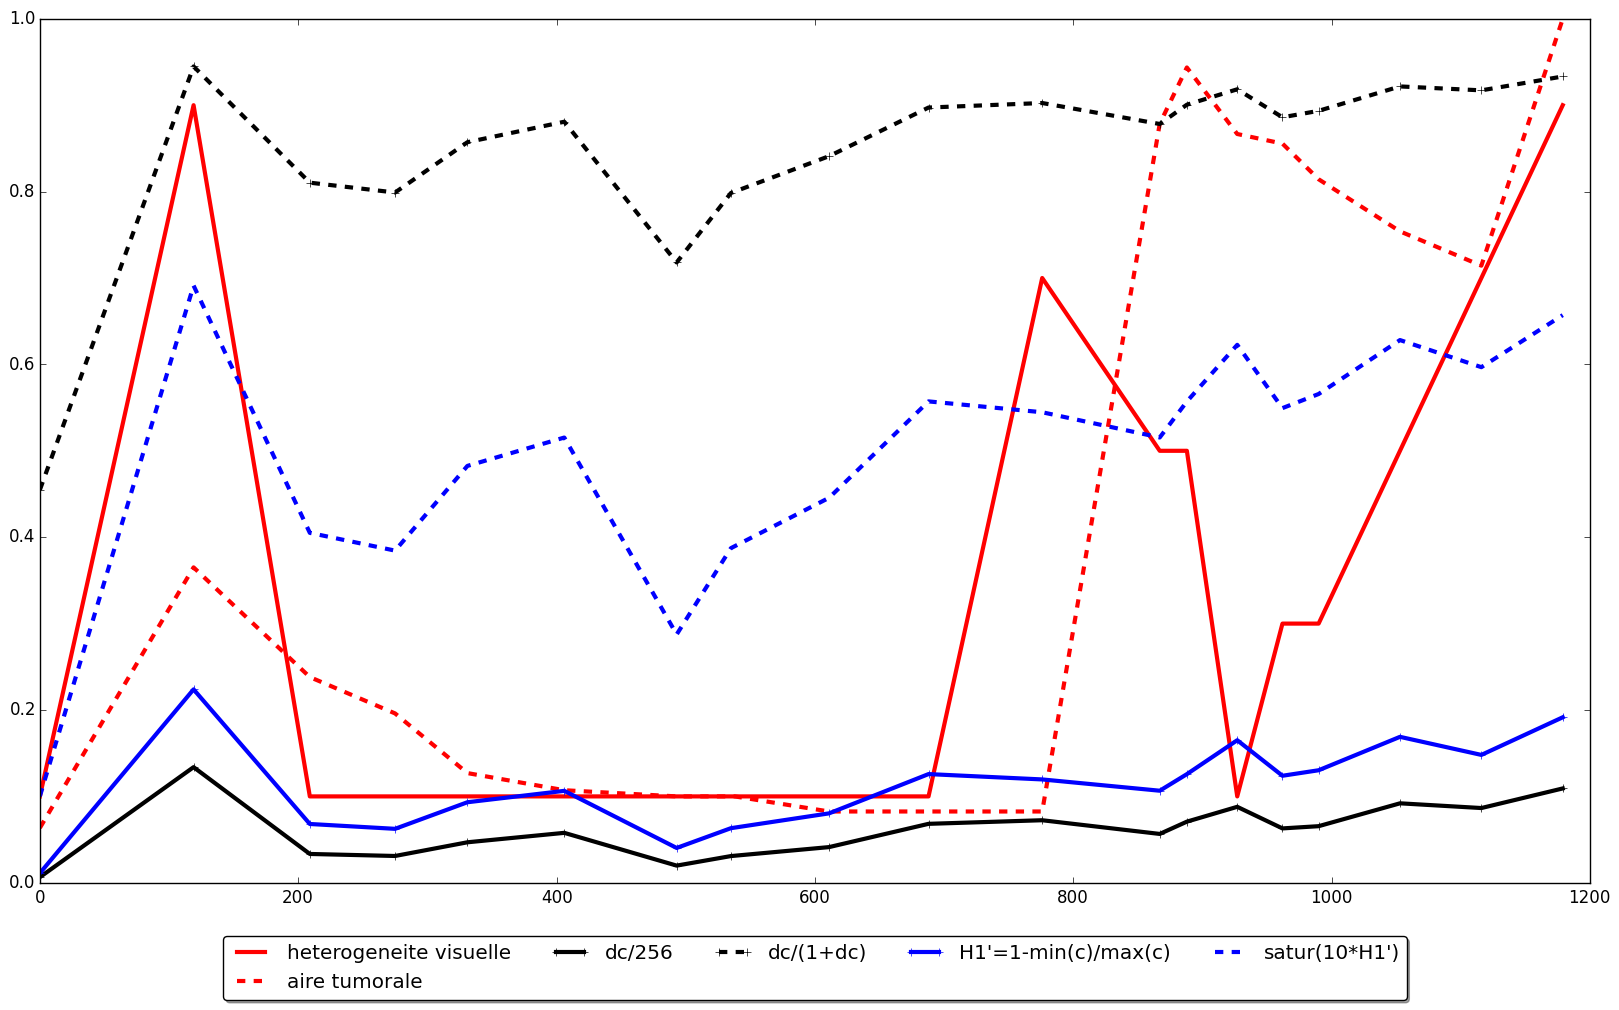
\includegraphics[width=0.49\textwidth]{graph_hetero/dcm_Nber/01-dc}}\ 
%\subfloat[\label{fig:critere_dh}Critères basés sur $\Delta h$]{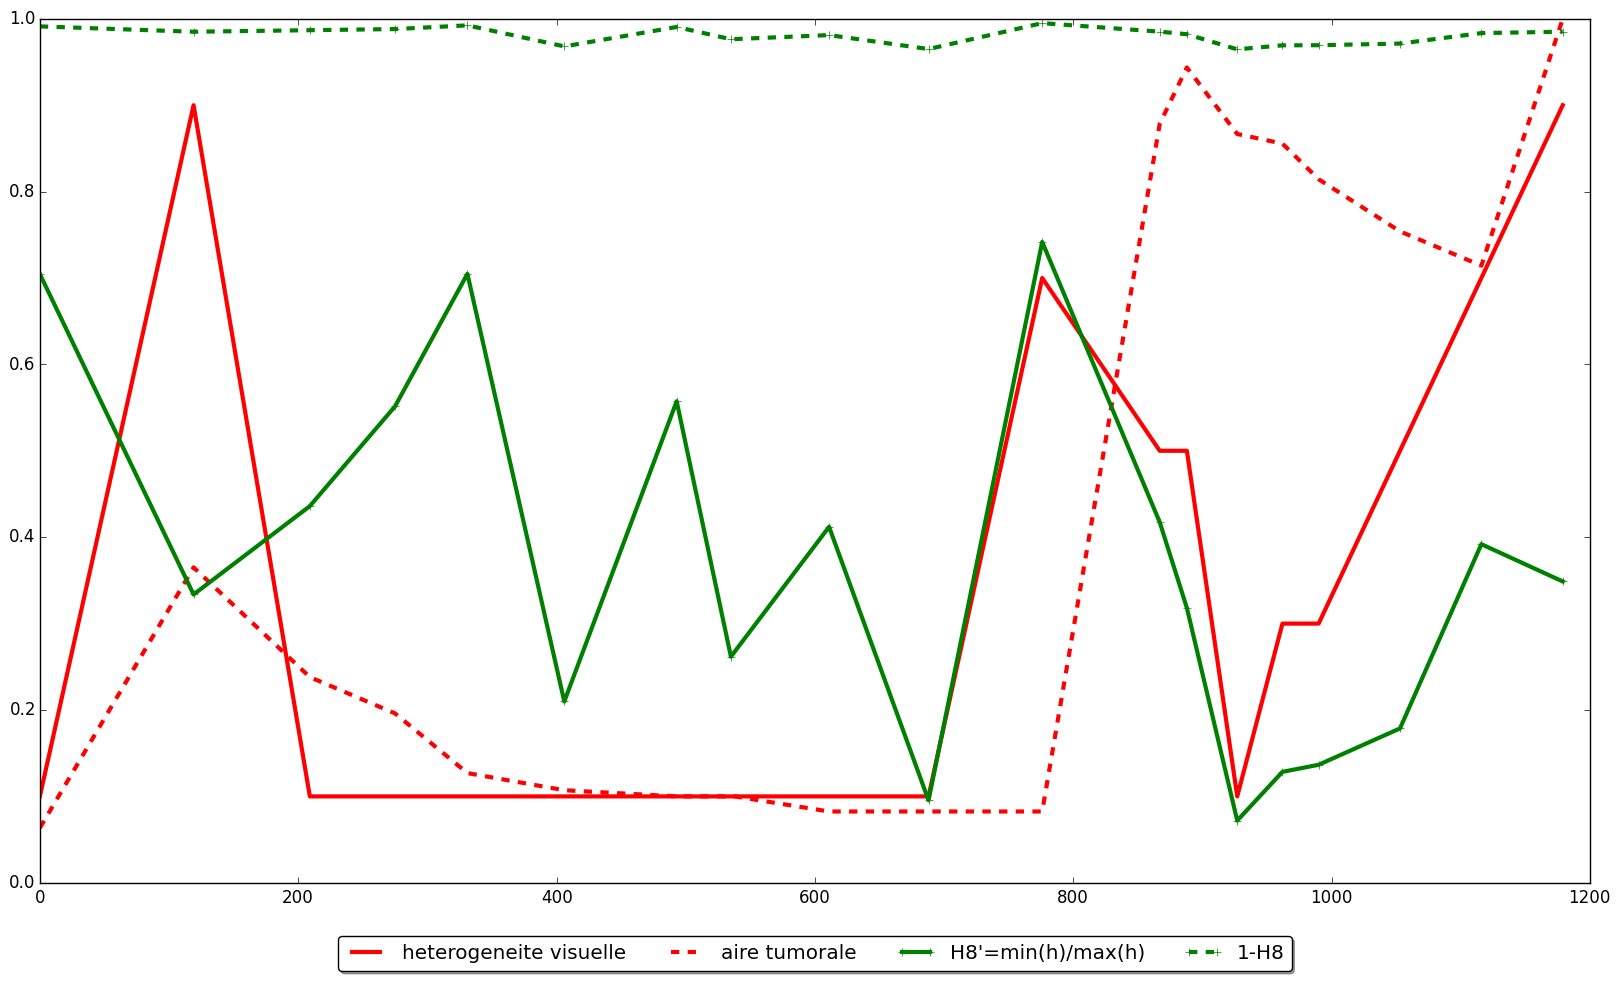
\includegraphics[width=0.49\textwidth]{graph_hetero/dcm_Nber/02-dh}}\\
%\subfloat[\label{fig:critere_dw}Critères basés sur $\Delta w$]{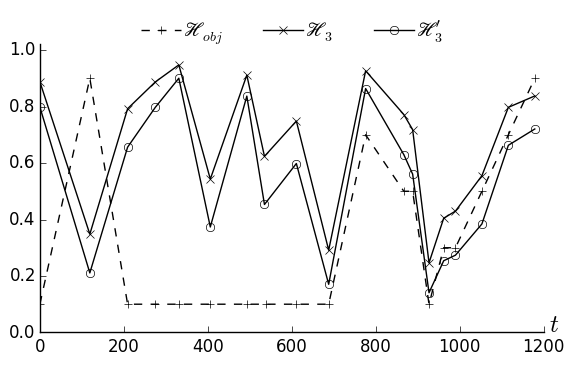
\includegraphics[width=0.49\textwidth]{graph_hetero/dcm_Nber/02_2-dw}}\ 
%\subfloat[\label{fig:critere_dc_sur_dh}Critères basés sur la pente $\dfrac{\Delta c}{\Delta h}$]{
%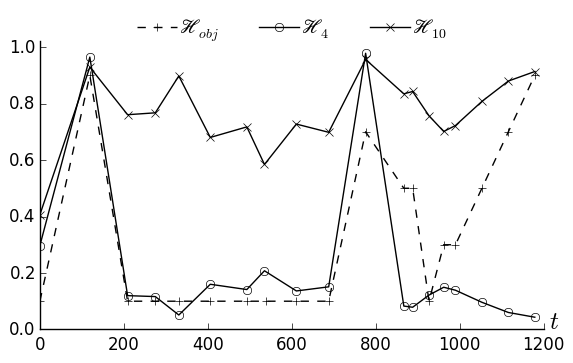
\includegraphics[width=0.49\textwidth]{graph_hetero/dcm_Nber/03-atan(dc_sur_dh)}}
%\caption{\label{fig:premiers_criteres}Premiers critères}
%\end{figure}
%
%%\begin{figure}[htpb]
%%\centering
%%%\subfloat[\label{fig:critere_dc_sur_dh}Critères basés sur la pente $\dfrac{\Delta c}{\Delta h}$]{
%%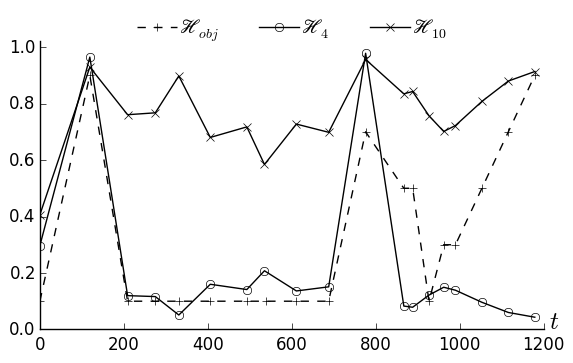
\includegraphics[width=0.70\textwidth]{graph_hetero/dcm_Nber/03-atan(dc_sur_dh)}
%%%}
%%\caption{\label{fig:critere_dc_sur_dh}Critères basés sur la pente $\Delta c / \Delta h$}
%%\end{figure}
%
%
%Notons que les ratios~$Qc, Qh$ et~$Qw$ sont par définition entre~0 et~1. 
%Pour les quantités~$\Delta h$ et~$\Delta w$ la propriété suivante nous permet aussi d'assurer la même condition.
%
%\begin{prop}
%\label{prop:bornitude_difference}
%Soit l'intervalle $I=]0,a[$ avec $a>0$. Alors~:
%\begin{equation}
%\forall (x,y)\in I^2, |x-y| < a - \min(x,y).
%\end{equation}
%En particulier, on a : $\forall (x,y)\in I^2, |x-y| < a$.
%\end{prop}
%La démonstration de cette propriété est quasiment immédiate par disjonction des cas $x=y$, $x<y$ et $x>y$.  
%
%Ainsi, par cette propriété, comme les poids~$w_i$ sont compris entre~0 et~1, alors~$\Delta w$ l'est aussi. 
%De même, comme $\sigma_i\geq 1$ alors, $h_i<1/\sqrt{2\pi}$ et donc $\Delta h<1/\sqrt{2\pi}$. 
%En ce qui concerne~$\Delta c$, rien n'assure qu'il soit dans l'intervalle~$[0;1]$. On le divisera par~256, pour également l'y ramener. De manière plus générale, pour garantir l'appartenance d'une quantité positive  à l'intervalle~$[0,1]$, on pourra lui appliquer la fonction de saturation~:
%\begin{equation}
%\label{eq:saturation_critere}
%\matheus{S}: x \longmapsto \dfrac{x}{1+x}.
%\end{equation}
%
%
%La Figure~\ref{fig:premiers_criteres}.abc montre l'évolution des quantités~\eqref{eq:H1}-\eqref{eq:H8bis} au cours du temps, avec application d'une saturation pour certaines. Tout d'abord, on peut remarquer les équivalences suivantes~:
%%\begin{equation}
%%\label{eq:equiv_diff_rapport}
%%\dfrac{\Delta c}{256} \simeq 1 - \dfrac{\min(c_1,c_2)}{\max(c_1,c_2)} \quad {\rm et } \quad \Delta w \simeq 1 - \dfrac{\min(w_1,w_2)}{\max(w_1,w_2)}.
%%\end{equation}
%\begin{equation}
%\label{eq:equiv_diff_rapport}
%%\dfrac{|\Delta c|}{256} \simeq 1 - Qc \quad {\rm et } \quad |\Delta w| \simeq 1 - Qw.
%\mathcal{H}_1 \simeq \mathcal{H}'_1  \quad {\rm et } \quad \mathcal{H}_3 \simeq \mathcal{H}'_3
%\end{equation}
%Ce comportement était attendu puisque les ratios varient de manière inverse aux différences. 
%Pour~$\mathcal{H}_8 (\sim |\Delta h|)$ et~$\mathcal{H}'_1 (\sim 1-Qh)$, on a visiblement pas d'équivalence stricte mais les variations du ratio semblent être une dilatation de celles de la différence comme le montre la courbe représentant~$1-10\mathcal{H}_8$ sur la Figure~\ref{fig:critere_dh}.
%
%On peut noter également que~$Qh$ et~$Qw$ sont très similaires et reproduisent assez bien la partie sur laquelle le patient est sous antiangiogénique. 
%
%%%De plus, bien que~$| \Delta c | / 256$ soit relativement bas, ses variations, si elles étaient dilatées,  pourrait s'approcher d'une description grossière de l'\hetero sur la partie avec imatinib.
%
%
%Outre ces similitudes, on remarque qu'aucune de ces quantités n'est pertinente pour décrire l'\hetero. Les quantités~$\Delta c/256$ et~$Qc$ n'excèdent pas 20\,\%. Sur la Figure~\ref{fig:critere_dc} sont aussi présentées deux dilatations de ces courbes. Même après dilatation, l'écart des centres ne semble pas pertinent pour décrire l'\hetero~: mis à part le premier pic qui semble capté, le reste de la courbe varie trop peu. 
%Pour ce qui est des quantités~$\mathcal{H}_8$, $\mathcal{H}'_8$, $\mathcal{H}_3$ et $\mathcal{H}'_3$ l'\hetero sur la partie angiogénique (après le jour~700) semble correctement captée. On ne peut pas en dire autant sur la première partie de la courbe. 
%
%
%Etudions donc de nouveaux critères. 
%Les prochains critères que nous allons étudier sont basés sur l'angle de la pente 
%\todo[noline]{Il s'agit de l'inverse de la pente}
%décrite entre le sommet des deux gaussiennes~:
%\begin{equation}
%\label{eq:critere_pente}
%\mathcal{H}_4 = \dfrac{1}{\pi} \atan \left( \dfrac{ \Delta c / 256 }{ \Delta h }  \right) + \dfrac{1}{2}
%\quad {\rm et } \quad
%\mathcal{H}_{10} = \dfrac{2}{\pi} \atan \left( \left| \dfrac{ \Delta c / 256 }{ \Delta h } \right| \right).
%\end{equation}
%\todo[noline]{l'arctangente ?}
%Notons que l'arctangente, n'est ni plus ni moins qu'une autre manière de saturer une quantité. En effet, comme le montre la Figure~\ref{fig:comp_saturation}, l'arctangente est proche de la saturation~$\matheus{S}$ définie par \eqref{eq:saturation_critere}. Ce graphique montre d'ailleurs également que d'autres saturations sont également possibles et équivalentes à celles utilisées.
%
%\begin{figure}
%\centering
%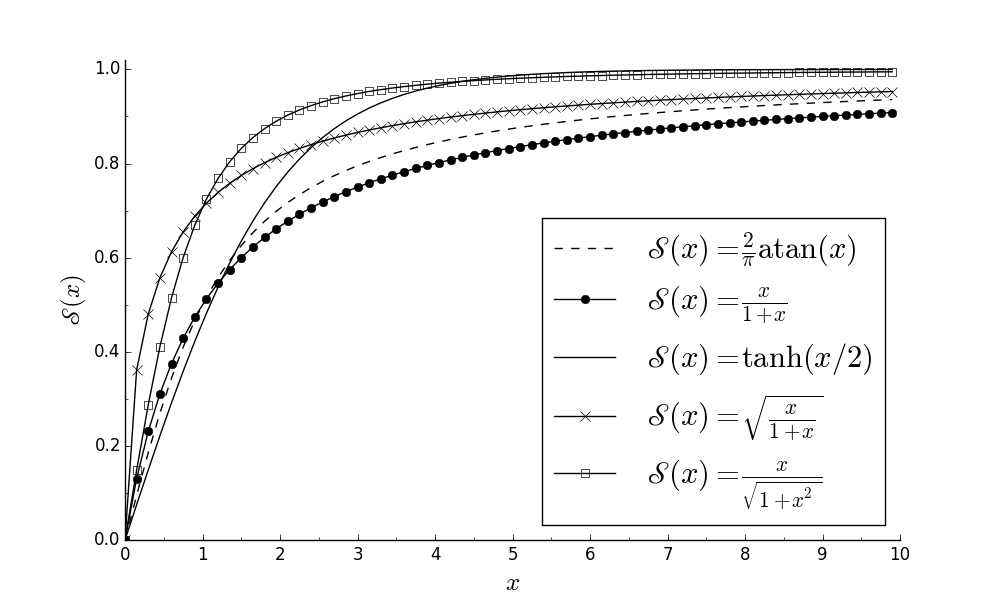
\includegraphics[width=0.75\textwidth]{comparaison_saturation.png}
%\vspace{-3mm}
%\caption{\label{fig:comp_saturation}Equivalence des différentes saturations}
%\end{figure}
%
%Sur la Figure~\ref{fig:critere_dc_sur_dh}, on peut voir que le critère~$\mathcal{H}_4$ recolle  relativement bien sur la partie correspondante au premier traitement, rechute incluse (jusqu'au jour 900). Cependant la recroissance finale n'est pas captée. En fait, $\mathcal{H}_4$ ne décrit pas l'\hetero. Il décrit le ratio proliférant sur nécrose. En effet~:
%\begin{myitemize}
%\item une pente positive va traduire qu'on a une majorité de proliférantes,
%\item une pente négative va traduire qu'on a une majorité de tissu nécrosé.
%\end{myitemize}
%Ce ratio est donc corrélé à l'\hetero, mais pas de manière linéaire puisqu'une tumeur avec 25\,\% de proliférant et 75\,\% de nécrose est aussi hétérogène qu'une tumeur présentant 75\,\% de proliférant et 25\,\% de nécrose. Nous avons donc besoin d'un critère indépendant du signe de la pente, tel~$\mathcal{H}_{10}$. Comme on peut le remarquer sur la Figure~\ref{fig:critere_dc_sur_dh}, ce critère n'est encore pas très convaincant en tant que quantificateur de l'\hetero... Les 3 pics à 90\,\% sont correctement captés, mais les parties basses traduisant des tumeurs bien homogènes ne sont pas bien décrites et ne diffèrent que trop peu des valeurs aux pics. D'autres critères doivent encore être explorés.
%
%\section{Critères basés sur la manière dont s'intersectent les gaussiennes}
%Avant de proposer divers autres critères, étudions de manière plus précise, la façon dont peuvent s'intersecter deux gaussiennes.
%%Avant de regarder quel critère qu'il soit, étudions l'ensemble des configurations possibles entre 2 gaussiennes.
%
%\subsection{Ensemble des configurations d'un mélange bi-gaussien \label{sec:config_gmm}}
%\begin{figure}[ht]
%\centering
%\subfloat[Cas avec 2 intersections, l'une se situant entre les centres des gaussiennes.]{
%\vspace{-3mm}
%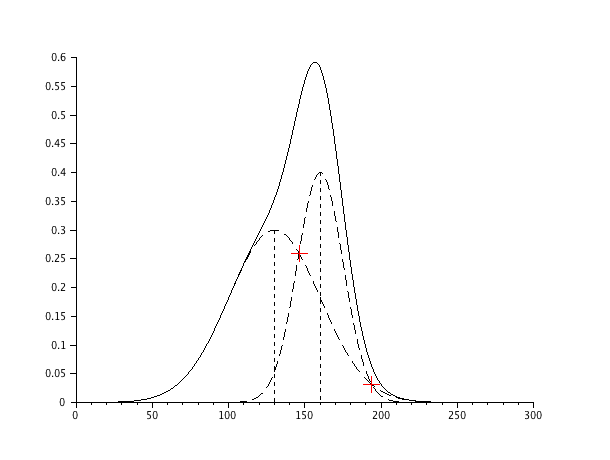
\includegraphics[width=.45\textwidth]{dessin_gauss/gmm_config1.png}}\qquad
%\subfloat[Cas avec 2 intersections, toutes les deux en dehors de l'intervalle défini par le centre des gaussiennes.]{
%\vspace{-3mm}
%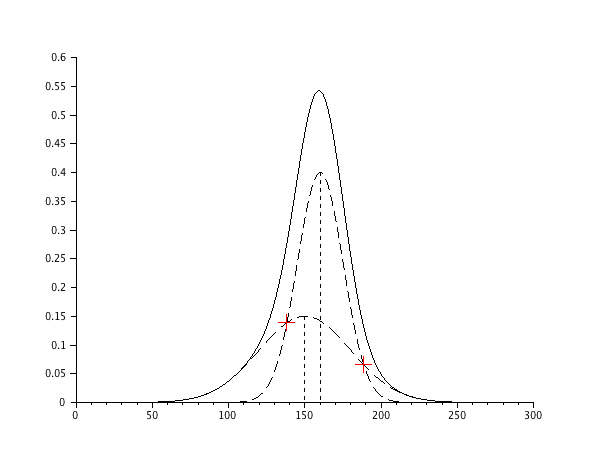
\includegraphics[width=.45\textwidth]{dessin_gauss/gmm_config2.png}}\\
%\subfloat[Cas avec un seul et unique point d'intersection (ici~$\sigma_1 = \sigma_2$).]{
%\vspace{-3mm}
%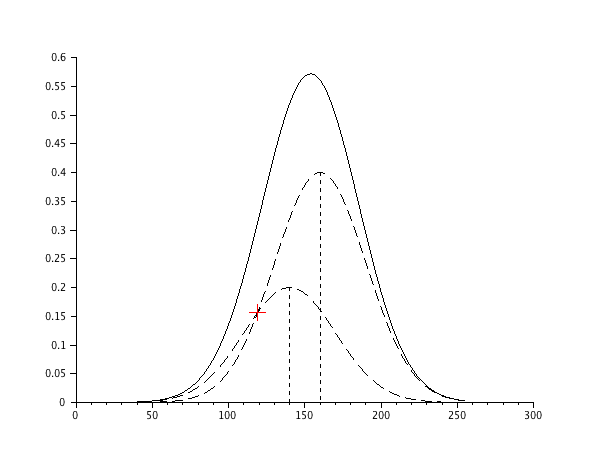
\includegraphics[width=.45\textwidth]{dessin_gauss/gmm_config3.png}}\qquad
%\subfloat[Cas sans aucun point d'intersection.]{
%\vspace{-3mm}
%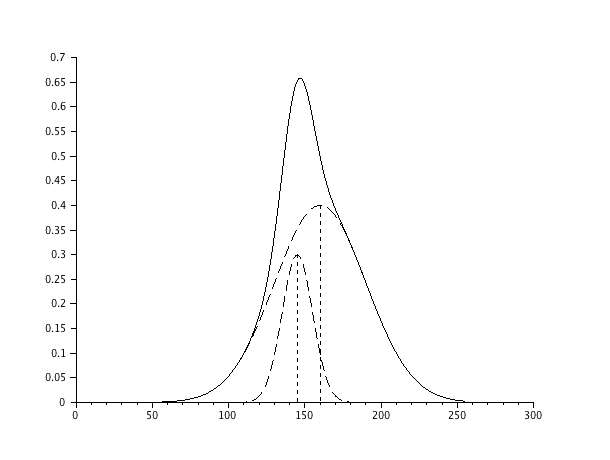
\includegraphics[width=.45\textwidth]{dessin_gauss/gmm_config4.png}}
%\caption{\label{fig:config_intersection_gaussienne}Ensemble des configurations avec 2 gaussiennes.}
%\end{figure}
%Comme le montre la Figure~\ref{fig:config_intersection_gaussienne}, deux gaussiennes ne s'intersectent pas nécessairement. De plus, il n'est pas obligatoire d'avoir un point d'intersection dont l'abscisse est située entre~$c_1$ et~$c_2$. Pour cela, résolvons l'équation suivante~:
%\begin{align*}
%g_1(x)=g_2(x) 
%& \Leftrightarrow h_1\exp \left(\frac{-1}{2} \left( \dfrac{x-c_1}{\sigma_1}\right)^2  \right) = h_2\exp \left(\frac{-1}{2} \left( \dfrac{x-c_2}{\sigma_2}\right)^2  \right), \\
%& \Leftrightarrow \ln h_1 - \dfrac{1}{2}\left( \dfrac{x-c_1}{\sigma_1} \right)^2 = \ln h_2 - \dfrac{1}{2}\left( \dfrac{x-c_2}{\sigma_2} \right)^2, \\
%& \overset{\sigma_i \neq 0}{\Leftrightarrow} 0 = \sigma_2^2 (x-c_1)^2 - \sigma_1^2 (x-c_2)^2 + 2\sigma_1^2\sigma_2^2 \ln( h_2 / h_1 ),
%\end{align*}
%qui amène à la résolution d'un polynôme du second degré en~$x$:
%\begin{equation}
%\begin{aligned}
%\label{eq:g1=g2}
%g_1(x)=g_2(x) \quad \Longleftrightarrow & \quad  Ax^2 + 2B'x + C =0 \\
%{\rm avec :} \quad &A=\sigma_2^2 - \sigma_1^2, \\
%& B'=c_2\sigma_1^2-c_1\sigma_2^2,\\
%& C= c_1^2\sigma_2^2-c_2^2\sigma_1^2 +  2\sigma_1^2\sigma_2^2 \ln( h_2 / h_1 ).
%\end{aligned}
%\end{equation}
%\paragraph{Cas particulier. \label{para:cas_partic_polynome}}
%Ecartons tout de suite le cas particulier~$\sigma_1=\sigma_2$. %, que l'on notera génériquement $\sigma$. 
%Dans ce cas, l'équation~\eqref{eq:g1=g2} se réécrit~:
%\begin{equation}
%\label{eq:g1=g2_cas_part}
%2\Delta c \; x + c_1^2-c_2^2 +  2 \sigma^2 \ln \big( (1-w) / w \big) = 0
%\end{equation}
%\begin{myitemize}
%\item Si de plus~$\Delta c=0$, alors \eqref{eq:g1=g2_cas_part} implique que~$h_1=h_2$, et donc les deux gaussiennes sont absolument identiques et superposées.
%\item Si~$\Delta c\neq0$, alors on a un seul et unique point de croisement, dont l'abscisse est~:
%\begin{equation}
%\label{eq:pt_croisement_unique}
%x=\dfrac{c_1+c_2}{2}-\dfrac{\sigma^2}{\Delta c}\ln \left( \dfrac{1-w}{w} \right).
%\end{equation}
%\end{myitemize}
%\paragraph{Cas général.} Il convient ici de calculer le discriminant réduit~:
%\begin{equation}
%\label{eq:discr_reduit}
%\Delta' := B'^2 - AC = \sigma_1^2 \sigma_2^2 \left[ (\Delta c)^2 - 2(\sigma_2^2-\sigma_1^2) \ln (h_2/h_1)  \right].
%\end{equation}
%Ce discriminant n'est pas nécessairement positif ! Donc il existe des cas où les gaussiennes ne s'intersectent pas. L'annexe~\ref{chap:anx_gmm} page~\pageref{chap:anx_gmm} présente une étude détaillée  du signe de ce discriminant (et donc de la manière dont peuvent s'intersecter 2 gaussiennes). On y montre que celui-ci est positif dans une large majorité de cas, ce qui appuie le fait qu'en pratique nous n'ayons jamais été confronté à des cas de gaussiennes ne s'intersectant pas (ou s'intersectant en un seul et unique point). 
%Outre le sommet des gaussiennes, ces points d'intersections sont de nouveaux points caractérisant le mélange. Voyons à présent s'ils peuvent conduire à un critère pertinent.
%
%\subsection{Etudes de différents critères}
%Différents critères seront étudiés dans cette section. Ils sont basés sur
%\begin{myitemize}
%\item l'intégrale commune aux deux gaussiennes
%\item la valeur de certains angles
%%\item des positions relatives de point ...
%\end{myitemize}
%
%\subsubsection{Critères basés sur la valeur d'angles particuliers.}
%\begin{figure}
%\centering
%\subfloat[{Cas où l'une des intersections se situe entre les centres des gaussiennes ($R_x \in [c_1;c_2] $).
%}]{\vspace{-3mm}
%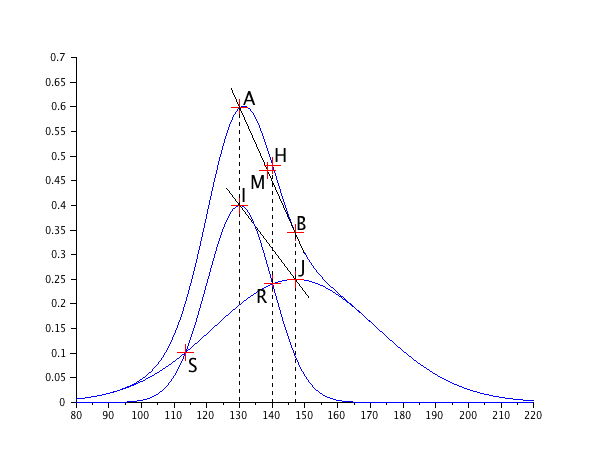
\includegraphics[width=.47\textwidth]{dessin_gauss/point_caracteristique_intersect_gauss.png}}\quad
%\subfloat[{Cas où les deux points d'intersection sont à l'extérieur ($R_x \notin [c_1;c_2] $).
%}]{\vspace{-3mm}
%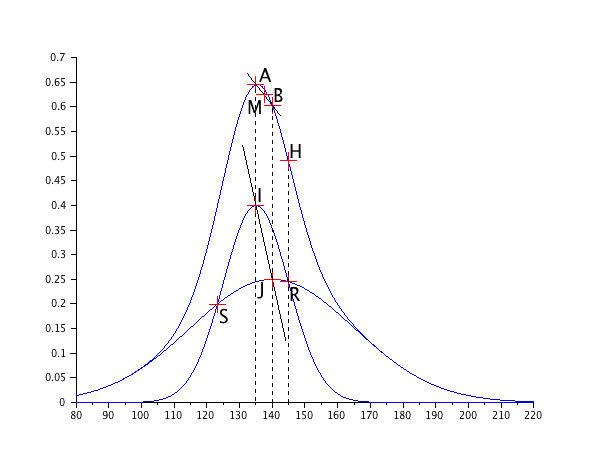
\includegraphics[width=.47\textwidth]{dessin_gauss/point_caracteristique_intersect_gauss_v2.png}}
%\caption{\label{fig:pts_carac_intersection_gaussienne}Points caractéristiques d'un mélange de deux gaussiennes.}
%\end{figure}
%
%Plutôt que de considérer seulement 2 points (le sommet de chaque gaussienne), élargissons notre éventail de points caractéristiques. La Figure~\ref{fig:pts_carac_intersection_gaussienne} présente l'ensemble des points utilisés dans les critères d'évaluation de l'\hetero de cette section. Cet ensemble de points n'existe que dans le cas où les gaussiennes possèdent 2 points d'intersections. Comme montré dans l'annexe~\ref{chap:anx_gmm}, les cas avec aucun ou un seul point d'intersection sont relativement marginaux (plus ou moins selon la valeur de~$\Delta c$ notamment). En plus des points~$I$ et~$J$ représentant le sommet de chaque composante ($I$ représentera toujours le sommet de la plus haute composante), on se servira de~$A$ et~$B$ qui représentent les valeurs du mélange gaussien en les centres des composantes~:~$c_1$ et~$c_2$ ($A$ ayant même abscisse que~$I$, et~$B$ même abscisse que~$J$). On notera également~$R$ et~$S$ les points d'intersections des composantes, $R$ étant le point le plus haut. On  considère également~$H$ positionné sur la courbe du mélange gaussien à la même abscisse que le point~$R$. Enfin, on note~$M$ le milieu de~$[AB]$. 
%
%
%On regardera ici les informations que peuvent fournir l'étude de différents angles. Un large spectre sera examiné~: $\widehat{ARB}$, $\widehat{MRB}$, $\widehat{MRA}$,  $\widehat{HRB}$, $\widehat{HRA}$, $\widehat{IRJ}$, $\widehat{MRJ}$, $\widehat{MRI}$, $\widehat{HRJ}$, $\widehat{HRI}$, $\widehat{IRB}$ et~$\widehat{ARJ}$. 
%On s'attend cependant à ce que certain d'entre eux soit équivalents, notamment ceux qui font intervenir des points sur la même verticale comme~$\widehat{HRA}$ et~$\widehat{HRI}$ par exemple avec \textit{a priori} une variation un peu plus importante du critère d'\hetero qui sera basé sur~$\widehat{HRA}$ que celui basé sur~$\widehat{HRI}$.
%
%Tous ces angles ne seront pas calculés. On ne s'intéressera uniquement qu'à leur cosinus qui se calcule aisément de la manière suivante avec le produit scalaire~:
%\begin{equation}
%\label{eq:cos_prod_scal}
%\cos(\widehat{BAC}) = \dfrac{ \overrightarrow{AB}.\overrightarrow{AC} }{ \| \overrightarrow{AB} \| \| \overrightarrow{AC} \|}.
%\end{equation}
%Notons que~:
%\begin{myitemize}
%\item Plus les angles définis ci-dessus sont petits, plus on s'attend à une tumeur homogène. Le critère d'\hetero doit donc avoir des variations inversées par rapport à celle du cosinus.
%\item Le critère doit être indépendant du signe de l'angle orienté. Tout critère basé sur le cosinus de l'angle respectera ceci, puisque le cosinus est une fonction paire.
%\item Le cosinus est à valeur dans [-1;1]. Le critère doit quant à lui être entre 0 et 1. Il faut donc adapter. Mais attention à la manière d'adapter. L'idée triviale de la valeur absolue ou du carré ne peut pas être appliquée ici. En effet, le signe de l'angle est sans importance mais le signe de son cosinus l'est ! Si l'angle est obtus (donc grand, ce qui traduirait une \hetero) le cosinus de l'angle est négatif et donc il ne faut surtout pas le ramener à son équivalent aigu ! De même on ne veut pas qu'un angle droit traduise un cas limite ($\mathcal{H} = 0$ ou 1). L'angle droit doit être le cas de transition entre l'angle obtus et l'angle aigu.
%\end{myitemize}
%On souhaite construire ici un critère qui varie de manière monotone en fonction de l'angle. Nous examinerons deux types d'adaptation d'échelle~:
%\begin{align}
%\mathcal{H}_5 (\theta) = &\dfrac{1-\cos \theta}{2} \\
%\mathcal{H}_6 (\theta) = &\sqrt{1-\left(  \dfrac{1+\cos \theta}{2}\right)^2}
%\end{align}
%\begin{figure}
%\subfloat[Avec adaptation~$\mathcal{H}_5$]{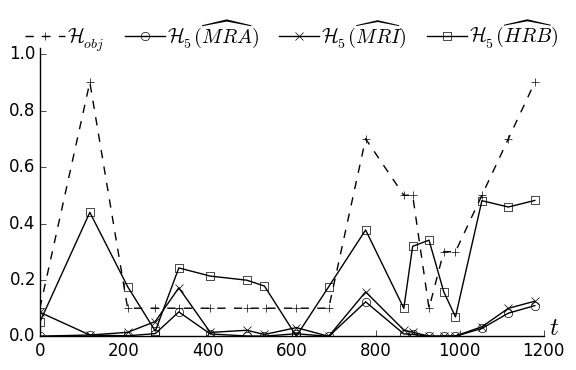
\includegraphics[width=0.49\textwidth]{graph_hetero/dcm_Nber/04-angle_complet_rescaleL1}}\ 
%\subfloat[Avec adaptation~$\mathcal{H}_6$]{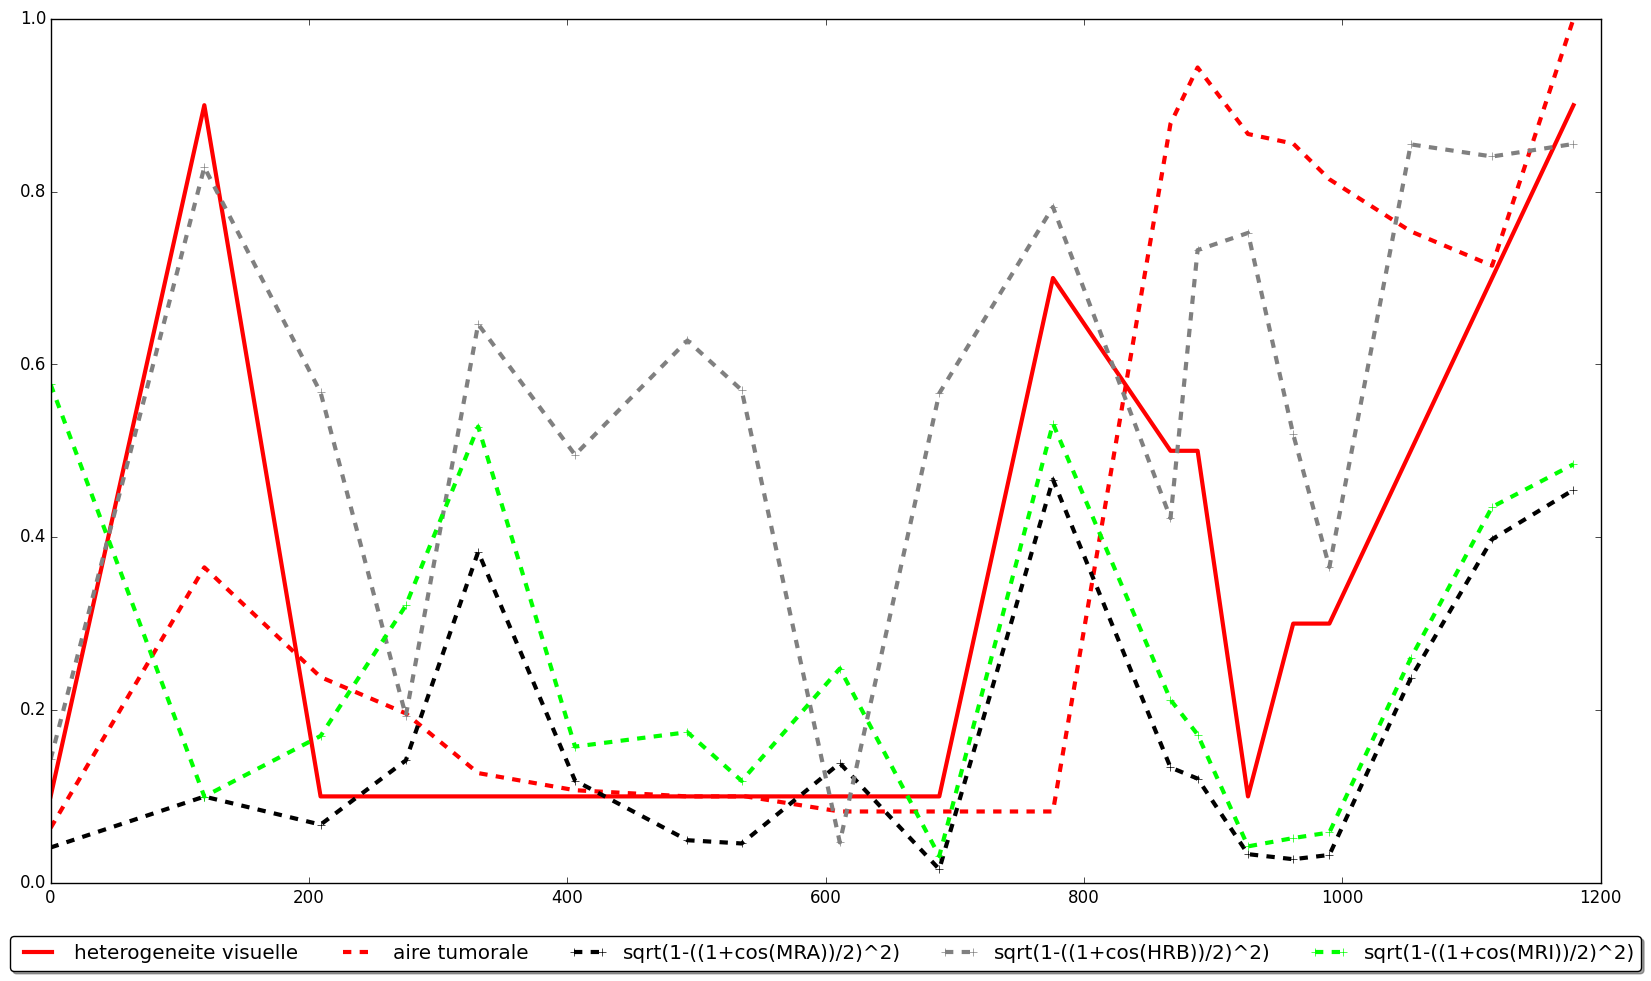
\includegraphics[width=0.49\textwidth]{graph_hetero/dcm_Nber/04-angle_complet_rescaleL2}}
%\caption{\label{fig:crit_hetero_angle}Critères basés sur des angles entre points particuliers de l'histogramme des niveaux de gris.}
%\end{figure}
%Pour beaucoup d'angles les résultats fournis sont insatisfaisants~: certains sont quasiment constant ($\mathcal{H}_{5,6}(\widehat{HRJ})$ par exemple), d'autres sont très chaotiques (comme~$\mathcal{H}_{5,6}(\widehat{ARB}$)). Sur la Figure~\ref{fig:crit_hetero_angle} sont présentés les critères d'\hetero restants (\ie non écartés pour les raisons précédentes). 
%Les critères basés sur l'angle~$\widehat{MRI}$ ou sur l'angle~$\widehat{MRA}$ semblent ne pas bien capturer le premier pic d'\hetero même si le second pic est capté ainsi que la remontée finale. Les critères basés sur l'angle~$\widehat{HRB}$ semblent eux bien capter les moments hétérogènes. Les pics d'\hetero sont cependant %assez faible et parfois 
%assez peu différents de certains passages homogènes... 
%%Les critères basés sur l'angle $\widehat{MRA}$ quant à eux, capturent très bien les deux premiers pics d'\hetero. Les passages homogènes sont également bien traduit (plateau lors du premier traitement, et pic descendant lors du second traitement). La recroissance finale de l'\hetero semble un peu plus laborieuse à capturer dans le cas du critère $\mathcal{H}_5$.
%Explorons à présent d'autres critères encore.
%
%\subsubsection{Critères basés sur des intégrales.}
%Dans cette section, on va s'intéresser à construire des critères basés sur des comparaisons  d'aires. Dans la section~\ref{sec:premier_essai_critere}, on a déjà examiné un critère qui compare l'aire des composantes entre elles. Il s'agit du critère~$Qw$, l'aire (l'intégrale) de la i-ème composante valant~$w_i$. 
%Ici, en observant les gaussiennes produites pour \Nber de plus près, on pourrait penser que l'aire commune aux deux gaussiennes (\cf schéma représentatif Figure~\ref{fig:gmm_aire_commune}) pourrait être un indicateur. Plus l'aire commune aux deux gaussiennes est élevée, plus les deux composantes seraient d'une certaine manière proche, et ainsi plus l'image serait homogène.  On s'intéresse ainsi aux critères suivants~:
%\begin{align}
%\mathcal{H}_9 =& 1 - \dfrac{ 1 }{\min(w_1,w_2)}\int \min(g_1(x),g_2(x)) \dx, \\
%\mathcal{H}'_9 =& 1-\int \min(g_1(x),g_2(x)) \dx.
%\end{align}
%\begin{figure}
%\subfloat[\label{fig:gmm_aire_commune}Schéma représentatif de l'aire commune à deux gaussiennes.]{
%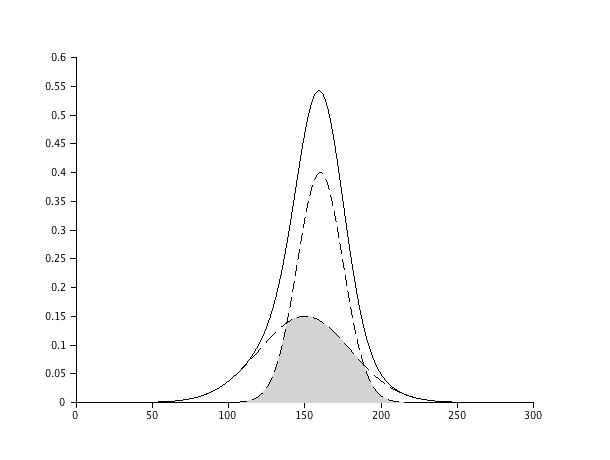
\includegraphics[width=.35\textwidth]{dessin_gauss/gmm_aire_commune.png}}
%\subfloat[\label{fig:crit_aire_commune}\Hetero fournit avec les critères~$\mathcal{H}_9$ et~$\mathcal{H}'_9$.]{
%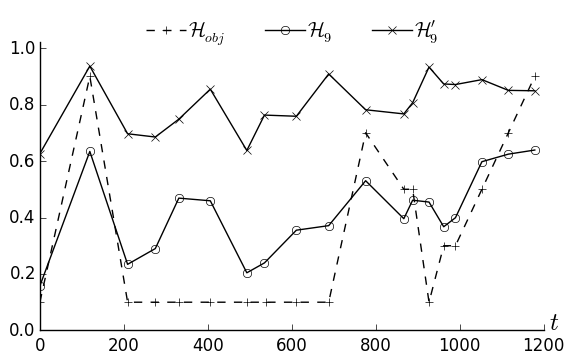
\includegraphics[width=.64\textwidth]{graph_hetero/dcm_Nber/05-integ_commune}}
%\caption{Critères basés sur l'aire commune aux deux gaussiennes~$\big($donnée par~: $\int_0^{255} \min \big(g_1(x),g_2(x) \big) \dx \big)$.}
%\end{figure}
%Les résultats pour ces deux critères sont présentés  Figure~\ref{fig:crit_aire_commune}. 
%Considérer l'aire commune relativement à l'aire de la plus petite des gaussiennes ($\mathcal{H}_9$) semble plus pertinent que de considérer l'aire commune seulement ($\mathcal{H}'_9$). Ce critère n'est pas des plus mauvais~: l'ensemble des moments hétérogènes est capturé (premier pic avant traitement jour~119, second et troisième pics avant les rechutes (jour~776 et~1116). Cependant les homogénéisations ne sont pas très bien capturées~: il y a notamment le plateau lors du premier traitement et le pic descendant lors du second traitement.



\section{Construction et analyse de critères divers}
Considérons désormais l'approximation en un mélange de deux gaussiennes des histogrammes de niveaux de gris provenant de nos images. Dans cette section, nous noterons\HH le critère d'\hetero que nous recherchons. 
La définition faite de l'\hetero dans la section précédente, nous invite à prendre en compte non pas les positions des gaussiennes, mais plutôt leur écart. Plus les gaussiennes sont similaires, et plus on tend vers un cas homogène. Partant de cette observation, 
des premiers critères naïfs ont été testés. Ces critères étaient basés sur des quantités simples~:  l'écart entre les centres des deux composantes ($\Delta c$) notamment et/ou l'écart de leur poids  ($\Delta w$) et/ou encore l'écart de leur hauteur ($\Delta h$). Bien que ces quantités ne se soient pas révélées être de bonnes traductrices de l'\hetero, elles m'ont permises d'aborder les questions suivantes~:
Comment parvenir à un critère\HH allant de 0 à 1 ? Comment bien normaliser les quantités intervenant dans le calcul de\HH ? Dans les cas où la normalisation des paramètres ne suffit pas à garantir l'appartenance de\HH à l'intervalle $[0;1]$, quelle saturation employer ? 

\begin{figure}
\centering
\subfloat%[Ensemble des points utilisés pour étudier la proximité de deux gaussiennes.  ]
[\label{fig:pts_carac_intersection_gaussienne}Position relative de points caractéristiques d'un mélange de deux gaussiennes]
{\vspace{-3mm}
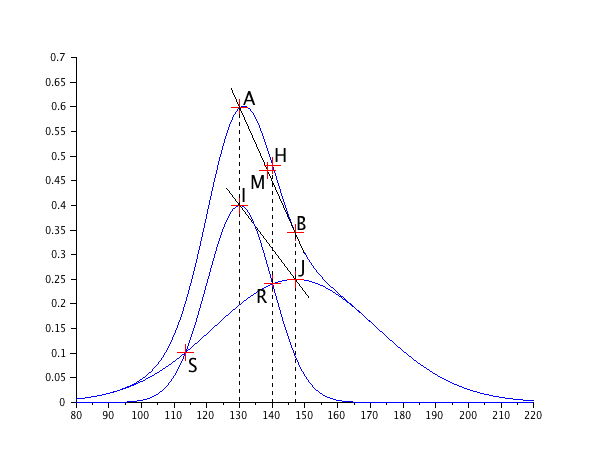
\includegraphics[width=.49\textwidth]{dessin_gauss/point_caracteristique_intersect_gauss.png}} 
\subfloat[\label{fig:aire_commune_gaussienne} Aire commune aux deux gaussiennes %~$\big($donnée par~: $\int_0^{255} \min \big(g_1(x),g_2(x) \big) \dx \big)$
]{\vspace{-3mm}
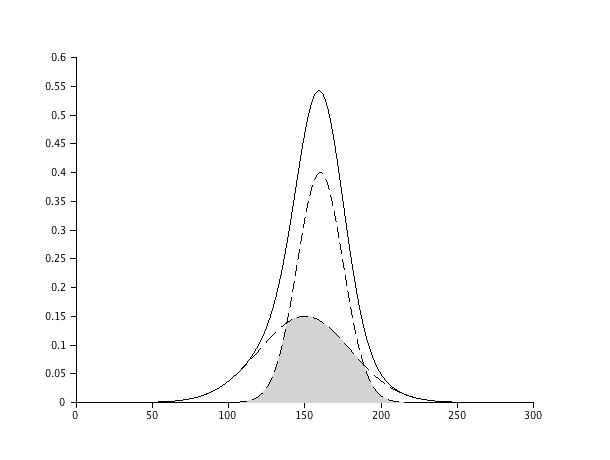
\includegraphics[width=.49\textwidth]{dessin_gauss/gmm_aire_commune.png}}
\caption{Caractérisation de la proximité des deux composantes gaussiennes}
\end{figure}


D'autres critères ont alors ensuite été essayés, basés sur :
\begin{myitemize}
\item la pente définie par le sommet des 2 composantes gaussiennes
\item ou la valeur de certains angles caractéristiques (en se servant de la position des points caractéristiques des deux composantes, \cf Figure~\ref{fig:pts_carac_intersection_gaussienne})
\item ou encore l'aire commune aux deux composantes (\cf Figure~\ref{fig:aire_commune_gaussienne})
\end{myitemize}
Beaucoup de difficultés ont été rencontrées pour construire un bon critère. Selon les choix réalisés, nous pouvons rapidement tomber dans le cas où\HH est 
\begin{myitemize}
\item soit quasiment constant avec une variation ne dépassant pas les 10 ou 15\% autour de la valeur moyenne
\item soit très chaotique, avec des variations que nous ne pourrions pas justifier.
\end{myitemize}
Dans les cas où les variations sont acceptables (ni trop faibles, ni chaotiques), faut-il encore que\HH recolle à la fonction objectif \ie qu'elle reproduise bien, au moins de manière qualitative, les différentes phases \heterogenes et homogènes constatées sur les scanners. % (pour ce qui est du quantitatif, on peut s'attendre à ce que les valeurs de la fonction objectif fixées de manière heuristique)


\section{Critère retenu}
\begin{figure}
\centering
\subfloat[\label{fig:pente_gaussienne_identique_a} Cas clairement \heterogene ]{
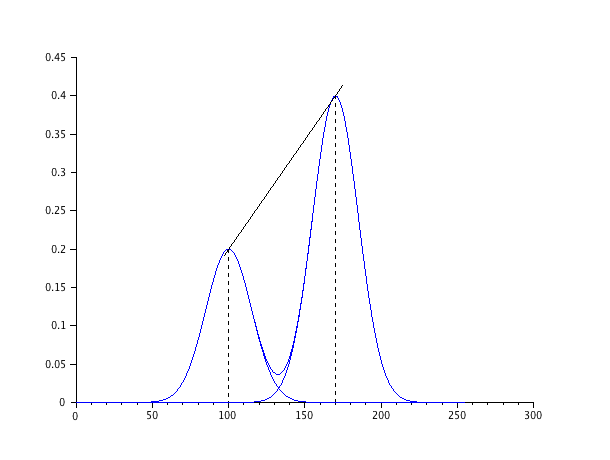
\includegraphics[width=.49\textwidth]{dessin_gauss/gmm_pente1a.png}
}
\subfloat[\label{fig:pente_gaussienne_identique_b} Cas plutôt homogène]{
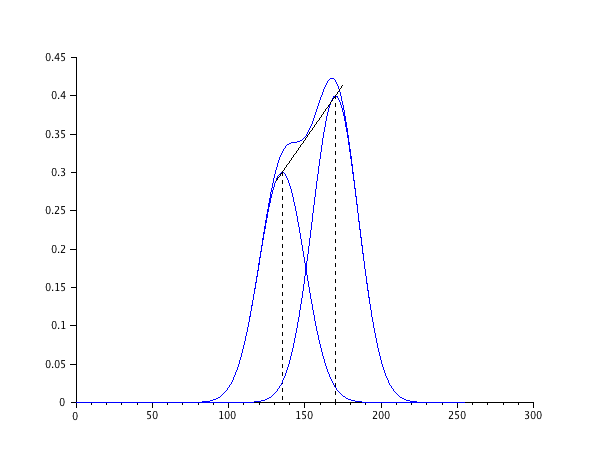
\includegraphics[width=.49\textwidth]{dessin_gauss/gmm_pente1b.png}
}
\caption{\label{fig:pente_gaussienne_identique}Deux configurations très différentes mais fournissant la même pente entre les gaussiennes.}
\end{figure}

L'idée de ce dernier critère m'est venue %de la constatation suivante, 
en repartant du critère  %$\mathscr{H}_{10}$ 
basé sur la pente décrite entre le sommet des gaussiennes. Sur la Figure~\ref{fig:pente_gaussienne_identique} sont présentées deux configurations très différentes, mais fournissant la même pente. Pourtant la Figure~\ref{fig:pente_gaussienne_identique_a} est très clairement représentative d'une image \heterogene alors que la Figure~\ref{fig:pente_gaussienne_identique_b} serait plutôt représentative de quelque chose d'homogène puisque l'approximation par une seule et unique gaussienne ne serait pas des plus mauvaises. 
Comment différencier ces deux cas ? Cet exemple mis en exergue nous invite à dire que~$\Delta c$ doit avoir plus de poids que~$\Delta h$ dans le calcul du critère\HH. %l'\hetero. 
%Ainsi, j'ai décidé de regarder le critère suivant~:
%\begin{equation}
%\label{eq:criteres_finaux}
%%\mathcal{H}_{11} =  \left| \dfrac{(\Delta c /256)^2}{\Delta w} \right| 
%%\quad {\rm et } \quad
%\mathcal{H}_{2} =  \left| \dfrac{(\Delta c /256)^2}{\Delta h} \right|
%\end{equation}
Ainsi regardons le critère suivant~:
\begin{equation}\label{eq:def_bon_critere}
\HH = \mathscr{S}(3\mathcal{H}) \quad \textrm{où} \quad \mathcal{H}=\left| \dfrac{(\Delta c /256)^2}{\Delta h} \right|,
\end{equation}
et où $\mathscr{S}$ est une fonction de saturation définie par~:
\begin{equation}
\mathscr{S} : x \mapsto \dfrac{x}{1+x}
\end{equation}

%%===
%Le seul bémol réside dans le fait que ce critère semble avoir des difficultés à monter vers les grandes \hetero. Multiplier ce critère par 3 semble corriger le problème. Mais pourquoi 3? 
Le facteur 3 dans la saturation a été considéré car sans celui-ci, le critère avait des difficultés à s'approcher de la valeur 1. Ce facteur n'a pas été choisi au hasard. %de la manière suivante. 
Si l'on regarde de plus près les histogrammes cliniques de \Nber, on peut remarquer qu'ils sont grossièrement tous compris dans l'intervalle~$[75;220]$. La longueur de cet intervalle est de 145, et non 256. Ainsi au lieu de diviser $\Delta c$ par 256, on peut le normaliser en le divisant par 145. Remarquons  alors que~:
\begin{equation}
\left(\frac{\Delta c}{145}\right)^2 \approx \left(\frac{\Delta c}{256/\sqrt{3}}\right)^2 =  3 \left(\frac{\Delta c}{256}\right)^2.
\end{equation}
%%===
Examinons à présent les résultats fournis par ce critère.

%\begin{figure}
%\centering
%\subfloat[\label{fig:critere_dc2_sur_dh} Critères basés sur $(\Delta c)^2 / \Delta h$ ]{
%\includegraphics[width=0.48\textwidth]{graph_hetero/dcm_Nber/06-dc2_sur_dh.png}
%}
%\subfloat[\label{fig:critere_dc2_sur_dw} Critères basés sur $(\Delta c)^2 / \Delta w$ ]{
%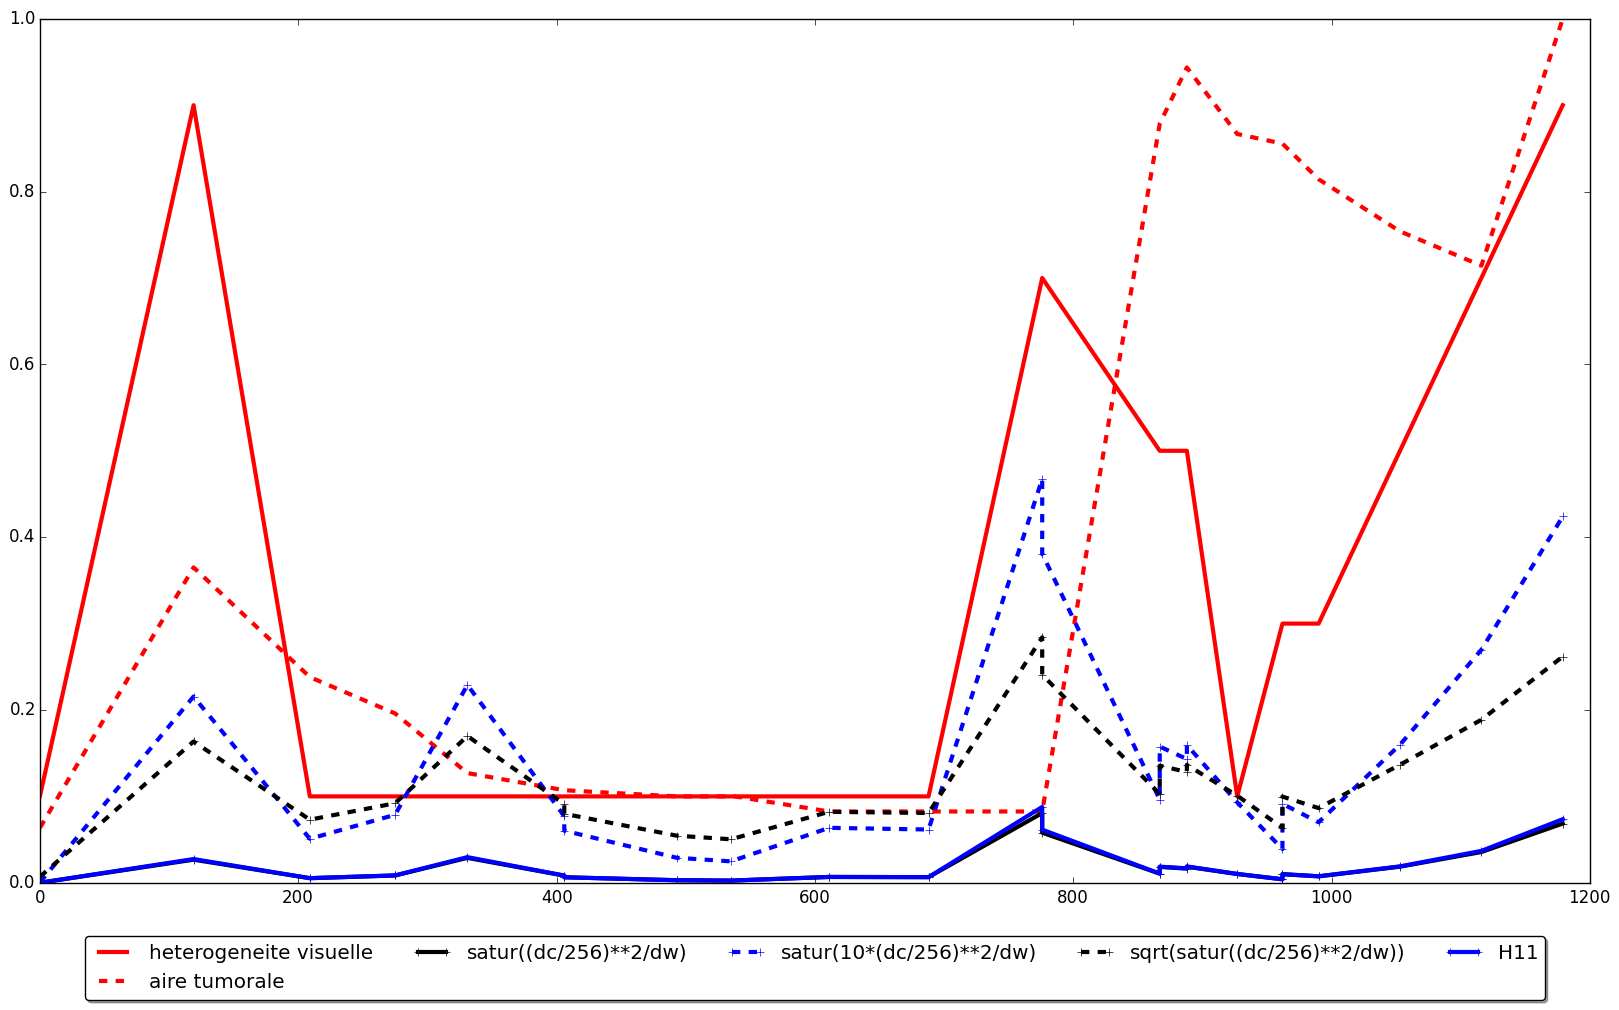
\includegraphics[width=0.48\textwidth]{graph_hetero/dcm_Nber/07-dc2_sur_dw.png}
%}
%\caption{\label{fig:critere_avec_dc2}Critères dans lesquels $\Delta c$ joue un rôle prépondérant.}
%\end{figure}
%
%\begin{figure}
%\centering
%\includegraphics[width=0.75\textwidth]{graph_hetero/dcm_Chen/06-dc2_sur_dh.png}
%\caption{\label{fig:critere_dc2_sur_dh_Chen} Critères basés sur $(\Delta c)^2 / \Delta h$ sur \Chen }
%\end{figure}

\begin{figure}[t]
\centering
\subfloat[\label{fig:critere_dc2_sur_dh_nber} \Nber ]{
\includegraphics[width=0.48\textwidth]{graph_hetero/dcm_Nber/06-dc2_sur_dh}
}
\subfloat[\label{fig:critere_dc2_sur_dh_chen} \Chen ]{
\includegraphics[width=0.48\textwidth]{graph_hetero/dcm_Chen/06-dc2_sur_dh}
}
\caption{\label{fig:critere_dc2_sur_dh}\Hetero clinique fournie par le critère~$\mathcal{H}_{2}$ dans lequel~$\Delta c$ joue un rôle prépondérant.}
\end{figure}


L'\hetero clinique, pour \Nber, fournie par le critère\HH est présentée sur la Figure~\ref{fig:critere_dc2_sur_dh_nber}. Ici, le critère reproduit bien les pics d'\heteros (jour~119 et jour~776). Le regain d'\hetero final, qui démarre avant la rechute au second traitement (jour 1100), et qui se poursuit pendant la rechute, est également bien capturé. Les phases homogènes sont également relativement bien reproduites. L'évaluation visuelle qui amenait à considérer l'\hetero constante du jour~209 au jour~688 est ainsi précisée par le critère. Manifestement le jour~331 est donc légèrement plus \heterogene. 
%Notons que bien qu'écartés, plusieurs autres critères (notamment~$\mathcal{H}_{10}$ et~$\mathcal{H}_6(\widehat{MRA})$) 
%avaient aussi capté cette subtilité. 
Enfin la forte homogénéisation causée par le second traitement est également bien traduite. 
Nous avons donc trouvé un critère qui semble quantifier de manière acceptable l'\hetero clinique de \Nber. Cela dit ce critère a été construit dans ce but. Afin de le valider, regardons ce qu'il en est sur notre second patient~: \Chen.


L'\hetero clinique, pour \Chen, fournie par le critère\HH est présentée sur la Figure~\ref{fig:critere_dc2_sur_dh_chen}. Ici aussi, la retranscription est aussi tout à fait acceptable. Les phases où il y a regain d'\hetero sont toutes correctement décrites. Au tout début (jusqu'au jour~279) la métastase est très petite. Il est donc difficile d'apprécier visuellement l'\hetero. De plus, le quantificateur sera aussi plus sensible aux erreurs dues au contourage. La tendance réelle à une baisse de l'\hetero est tout à fait plausible. D'autant plus que c'est le comportement attendu lorsque le traitement agit de manière efficace~: l'ensemble de la métastase tend à se nécroser, et donc le tout s'homogénéise. 
L'homogénéisation lors du second traitement est également très bien capturée (autour du jour 1200). 
Les pics d'\hetero (du jour 800 à 1100 puis remontée finale) sont aussi bien traduits. 
%De même que pour \Nber, le critère~$\matheus{S}(3\mathscr{H}_2)$ s'approche plus de l'objectif que le critère~$\matheus{S}(\mathscr{H}_2)$. 
Bien qu'étant plus larges, les histogrammes cliniques de \Chen n'occupent pas l'ensemble de l'intervalle~$[0;256]$. Si nous nous restreignons à l'intervalle~$[75;220]$, ce qui est en dehors reste très marginal et la multiplication par~3 se justifie également ici. 


\section{L'\hetero sur les simulations numériques}

Maintenant que nous avons un critère qui décrit correctement l'\hetero clinique (d'une métastase à partir de l'imagerie médicale), testons le %faisons parler ce critère 
sur nos simulations numériques. 
En ce qui concerne cet aspect, les images de synthèse (dont le procédé est détaillé dans le Chapitre~\ref{chap:optim_grey}) résultants des simulations numériques dépendent de 3 paramètres~: $\tau_N, \tau_P$ et~$\tau_S$ qui représentent les niveaux de gris associés à chacune de nos populations de notre modèle EDP. Ainsi, pour une simulation numérique donnée, il n'y a pas unicité de l'image produite en niveaux de gris, et donc non unicité de l'histogramme. Tout dépend de ces 3 paramètres. 
Dans un premier temps, nous examinerons % ce que cela donne 
les résultats fournis 
avec les valeurs heuristiques considérées  dans la première partie de ce manuscrit~: $\tau_N=38, \tau_P=166$ et~$\tau_S=204$. 
Dans un second temps, nous pourrons faire varier ces paramètres pour examiner l'influence de ceux-ci sur l'\hetero numérique. Nous examinerons notamment ce qui est produit avec les niveaux de gris optimaux du chapitre précédent. 

%On ne montrera ici que l'\hetero numérique de \Nber. Celle de \Chen n'a absolument aucune chance d'être correctement reproduite pour la simple et bonne raison que le premier scan est très \heterogene, alors que notre condition initial dans le modèle numérique est complètement homogène. Il faudrait prendre une condition initiale plus en relation avec l'image médicale, à minima une condition initiale qui présenterait le même niveaux d'\hetero pour pouvoir poursuivre l'étude avec ce patient.

\subsection{\Nber}

\begin{figure}
\centering
\includegraphics[width=0.75\textwidth]
%{graph_hetero/simu_Nber_N38_P166_S204/06-dc2_sur_dh.png}
{graph_hetero/simu_Nber_N25_P143_S197/06-dc2_sur_dh.png}
\caption{\label{fig:hetero_nber_simu}\Hetero numérique pour \Nber\ -- $\tau_N=38, \tau_P=166$ et~$\tau_S=204$. La fonction objectif\HHobj de l'\hetero clinique est rappelée ici à titre de comparaison.}
\end{figure}

L'\hetero numérique de \Nber est présentée sur la Figure~\ref{fig:hetero_nber_simu}. 
La fonction objectif pour l'\hetero clinique %ainsi que l'évolution de l'aire tumorale sont
est ici rappelée sur ce graphique à titre comparatif. La phase avec imatinib est  correctement décrite~:
\begin{myitemize}
\item Présence d'un pic d'\hetero jour~119.
\item Décroissance de l'\hetero lorsque l'imatinib agit de manière efficace du jour~200 au jour~700.
\item Saut important de l'\hetero qui grandit, autour du jour~800, juste avant la recroissance de l'aire tumorale.
\end{myitemize}
En ce qui concerne la partie avec sunitinib, au début de l'administration du traitement (jour 888) l'\hetero décroît. Cependant~:
\begin{myitemize}
\item La recroissance de l'\hetero numérique a lieu un peu tôt par rapport à celle constatée cliniquement et est assez abrupte.
\item Sur la partie finale (lors de la rechute au sunitinib, après le jour~1116), l'\hetero numérique décroît alors que celle clinique continue d'augmenter. 
\end{myitemize}
En ce qui concerne le deuxième point, cela peut venir soit de la manière dont  l'\hetero est calculée, soit du modèle EDP lui-même qui ne retranscrirait pas bien l'évolution de l'\hetero. La Figure~\ref{fig:baisse_hetero_fin_simu} tend à dire que c'est plutôt le modèle EDP qui est responsable puisque l'image scanner reconstruite à partir de la la simulation numérique est 
% beaucoup 
plus \heterogene jour~1120 qu'au jour~1227. 
En effet, le contraste (écart d'intensité) entre les deux masses dominantes (pourtour et intérieur de la tumeur) 
est beaucoup plus important jour~1120 que jour~1227. De plus le rapport du volume de ces dominantes est beaucoup plus proche de 1 au jour~1120 qu'au jour~1227 (si le ratio est égal à 1 alors les 2 nuances de gris occupent chacune un volume égal). Ces impressions visuelles sont confirmées par les histogrammes également présentés sur la Figure~\ref{fig:baisse_hetero_fin_simu}. 
Tout ceci renforce donc l'idée que l'image numérique du jour~1120 est plus \heterogene que celle du jour~1227 et notre critère le traduit bien. Le modèle EDP semblerait donc bien retranscrire globalement les différentes phases  \heterogenes /homogènes au moins durant le premier traitement. Après le jour~950, l'\hetero numérique ne semble plus correctement  décrire l'\hetero clinique. Ceci n'est guère surprenant. % au vu desq arguments suivants~:
%\begin{myitemize}
%\item 
En effet, un grand nombre d'itérations est effectué dans le calcul numérique pour parvenir au temps final. Les erreurs se cumulant au fil des itérations, il n'est donc pas étonnant qu'à un moment donné l'\hetero numérique ne recolle pas complètement à l'\hetero clinique.
%\item Ici nous étudions les cas avec seulement 3 populations de cellules proliférantes. Cependant les résistances au traitement ne sont pas limités à deux, le phénomène contrôle puis rechute peut se reproduire un certain nombre de fois tout en variant les traitements. Les populations mutantes sont donc plus nombreuses. Ainsi, à la fin de la simulation, l'hypothèse de ces 3 populations devient de plus en plus fausses car ces nouvelles
%\end{myitemize}


\begin{figure}
\centering
\subfloat[Jour~1120]
{\begin{tabular}{c}
\includegraphics[width=0.31\textwidth]
%%{simu/N38_P166_S204/fit_henbert_form3_seuil0.1/tumor086.png}\\
{simu/N38_P166_S204/fit_henbert_form3_seuil0.1/simu_contour086.png}\\
\includegraphics[width=0.31\textwidth]
%%{simu/N38_P166_S204/fit_henbert_form3_seuil0.1/histo/Nber_day1120(85).png}
{simu/N38_P166_S204/fit_henbert_form3_seuil0.1/histo/fit_histo085.png}
\end{tabular}}
\subfloat[Jour~1186]
{\begin{tabular}{c}
\includegraphics[width=0.31\textwidth]
%%{simu/N38_P166_S204/fit_henbert_form3_seuil0.1/tumor091.png}\\
{simu/N38_P166_S204/fit_henbert_form3_seuil0.1/simu_contour090.png}\\
\includegraphics[width=0.31\textwidth]
%%{simu/N38_P166_S204/fit_henbert_form3_seuil0.1/histo/Nber_day1186(90).png}
{simu/N38_P166_S204/fit_henbert_form3_seuil0.1/histo/fit_histo090.png}
\end{tabular}}
\subfloat[Jour~1227]
{\begin{tabular}{c}
\includegraphics[width=0.31\textwidth]
%{simu/N38_P166_S204/fit_henbert_form3_seuil0.1/tumor095.png}\\
{simu/N38_P166_S204/fit_henbert_form3_seuil0.1/simu_contour095.png}\\
\includegraphics[width=0.31\textwidth]
%%{simu/N38_P166_S204/fit_henbert_form3_seuil0.1/histo/Nber_day1227(94).png}
{simu/N38_P166_S204/fit_henbert_form3_seuil0.1/histo/fit_histo094.png}
\end{tabular}}
\caption{\label{fig:baisse_hetero_fin_simu} Evolution de l'\hetero numérique de \Nber du jour 1120 au jour 1227.}
\end{figure}


De plus les images numériques sont dépendantes du choix des niveaux de gris~$\tau_N$, $\tau_P$ et~$\tau_S$. Ce choix pourrait aussi être une source d'écart entre l'\hetero clinique et l'\hetero numérique.

%\subsection{Influence des niveaux de gris sur l'\hetero numérique}
\subsection{Robustesse du critère}
Examinons ici l'influence du choix de la paramétrisation de la reconstruction d'images scanners sur la quantification de l'\hetero. 
Cette paramétrisation consiste à choisir les trois niveaux de gris~$\tau_N$, $\tau_P$ et~$\tau_S$.  
La principale conséquence d'un changement de ces niveaux de gris est la dilatation de l'histogramme numérique résultant.  
Les variations de l'\hetero ne sont donc que peu dépendantes de ces paramètres. L'amplitude des variations pourra éventuellement être impactée mais le sens (et c'est cela qui nous intéresse) lui ne sera pas changé. 
Ceci est corroboré par les tests numériques, dont les résultats sont présentés sur la Figure~\ref{fig:impact_grey_lvl_on_hetero}. 
En effet, on remarque ici que toutes les courbes sont comparables. Comme différence, on pourra relever tout de même que plus~$\tau_N$ est écarté de~$\tau_P$, plus les variations de l'\hetero numérique sont importantes. Ceci est notamment visible lors de la rechute à l'imatinib, entre les jour~776 et~888 où le pic descendant de l'\hetero numérique est plus prononcé si~$\tau_P-\tau_N$ est grand. Ceci est conforme à ce que l'on pouvait attendre, puisque cette différence va impacter directement la position des gaussiennes sur l'histogramme, position relative en grande partie donnée par~$\Delta c$ qui intervient dans le calcul de notre critère de l'\hetero numérique. 

%\begin{figure}[h]
%\centering
%\subfloat[$\tau_N=23, \tau_P=142$ et $\tau_S=215$]
%{\includegraphics[width=0.48\textwidth]
%{graph_hetero/simu_Nber_N23_P142_S215/06-dc2_sur_dh.png}}
%\subfloat[$\tau_N=30, \tau_P=122$ et $\tau_S=215$]
%{\includegraphics[width=0.48\textwidth]
%{graph_hetero/simu_Nber_N30_P122_S215/06-dc2_sur_dh.png}}\\
%\subfloat[$\tau_N=26, \tau_P=127$ et $\tau_S=215$]
%{\includegraphics[width=0.48\textwidth]
%{graph_hetero/simu_Nber_N26_P127_S215/06-dc2_sur_dh.png}}
%\subfloat[$\tau_N=36, \tau_P=142$ et $\tau_S=215$]
%{\includegraphics[width=0.48\textwidth]
%{graph_hetero/simu_Nber_N36_P142_S215/06-dc2_sur_dh.png}}
%\caption{\label{fig:impact_grey_lvl_on_hetero} Influence du choix des niveaux de gris $\tau_N, \tau_P$ et $\tau_S$ sur l'\hetero numérique.}
%\end{figure}

\begin{figure}[h]
\centering
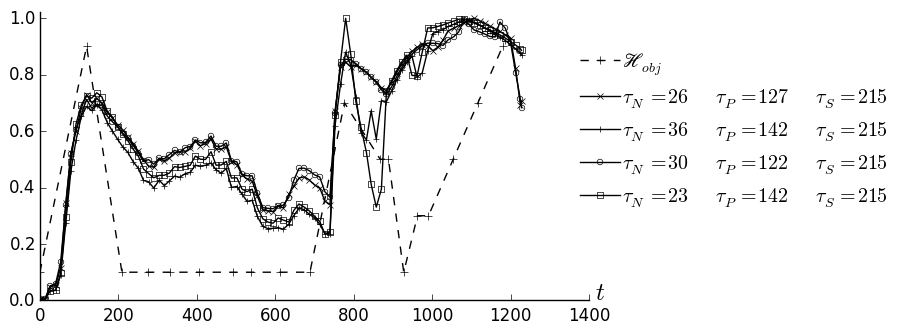
\includegraphics[width=\textwidth]{graph_hetero/simu_Nber_dc2_sur_dh_sensibilite_nvx_gris.png}
\caption{\label{fig:impact_grey_lvl_on_hetero} Influence du choix des niveaux de gris $\tau_N, \tau_P$ et $\tau_S$ sur l'\hetero numérique donnée par\HH (\cf équation~\eqref{eq:def_bon_critere}). --  La fonction objectif\HHobj de l'\hetero clinique est rappelée ici à titre de comparaison.}
\end{figure}

\subsection{\Chen}
%On ne montrera ici que l'\hetero numérique de \Nber. Celle de \Chen n'a absolument aucune chance d'être correctement reproduite pour la simple et bonne raison que le premier scan est très \heterogene, alors que notre condition initial dans le modèle numérique est complètement homogène. Il faudrait prendre une condition initiale plus en relation avec l'image médicale, à minima une condition initiale qui présenterait le même niveaux d'\hetero pour pouvoir poursuivre l'étude avec ce patient.

\begin{figure}[h]
\centering
\includegraphics[width=0.75\textwidth]
%{graph_hetero/simu_Chen_N38_P166_S204/06-dc2_sur_dh.png}
%\caption{\label{fig:hetero_chen_simu}\Hetero numérique pour \Chen\ -- $\tau_N=38, \tau_P=166$ et~$\tau_S=215$. La fonction objectif\HHobj de l'\hetero clinique est rappelée ici à titre de comparaison. La simulation numérique ne reproduit ici pas du tout l'\hetero clinique.}
{graph_hetero/simu_Chen_N25_P143_S197/06-dc2_sur_dh.png}
\caption{\label{fig:hetero_chen_simu}\Hetero numérique pour \Chen\ -- $\tau_N=25, \tau_P=143$ et~$\tau_S=197$. La fonction objectif\HHobj de l'\hetero clinique est rappelée ici à titre de comparaison. La simulation numérique ne reproduit ici pas du tout l'\hetero clinique.}
\end{figure}

L'\hetero numérique de \Chen est présentée sur la Figure~\ref{fig:hetero_chen_simu}. Comme on peut le voir sur ce cas, l'\hetero  numérique n'est pas comparable à l'\hetero clinique. Il y a en fait assez peu de chance pour qu'il y ait recollement de ces deux courbes. En effet, le premier scanner de \Chen est très \heterogene, alors que notre condition initiale dans le modèle numérique est complètement homogène. Il faudrait prendre une condition initiale plus en relation avec l'image médicale, {\it a minima} une condition initiale qui présenterait le même niveau d'\hetero pour pouvoir poursuivre l'étude avec ce patient. 

Malgré cela, notons que le critère semble tout de même bien décrire l'\hetero numérique. 
% puisque
En effet, comme le montrent les images numériques présentées dans la Figure~\ref{fig:simu_complete_chen} de l'annexe~\ref{chap:anx_img_complement} (page~\pageref{fig:simu_complete_chen}), la simulation produit une tumeur quasi homogène jusqu'au jour~1100, puis une apparition brutale d'\hetero entre les jours~1100 et~1200 et enfin une baisse progressive de l'\hetero après le jour~1200. Le quantificateur de l'\hetero \HH traduit donc bien cela. Nous parvenons ici une nouvelle fois aux limites du modèle EDP, dont le choix de la condition initiale semble prépondérant.

\end{document}